%TODO: CORREGIR COMANDOS PARA QUE SE VEAN CON VERB
%TODO: INTENTAR QUITAR LA MORRAYA QUE NO SIRVA
%TODO: INTENTAR NO REPETIR TANTAS COSAS EN EL EJERCICIO 3
%TODO: REVISAR DOCUMENTO PARA FALLOS ORTOGRAFICOS/GRAMATICALES
\documentclass{article}
\usepackage[utf8]{inputenc}
\usepackage[spanish]{babel}
\usepackage{graphicx, graphics, float, hyperref}
\usepackage{listings, subcaption}
\usepackage[a4paper, total={6in, 10in}]{geometry}

\title{SSO Práctica 2 Sesión 1}
\author{Andrés Merlo Trujillo}
\date{}
\hypersetup{
    colorlinks=true,
    linkcolor=black,
}

\begin{document}

\maketitle

\tableofcontents

\newpage
%\addcontentsline{toc}{section}{Ejercicio 1}
%\section*{Ejercicio 1}
%\begin{figure}[H]
%    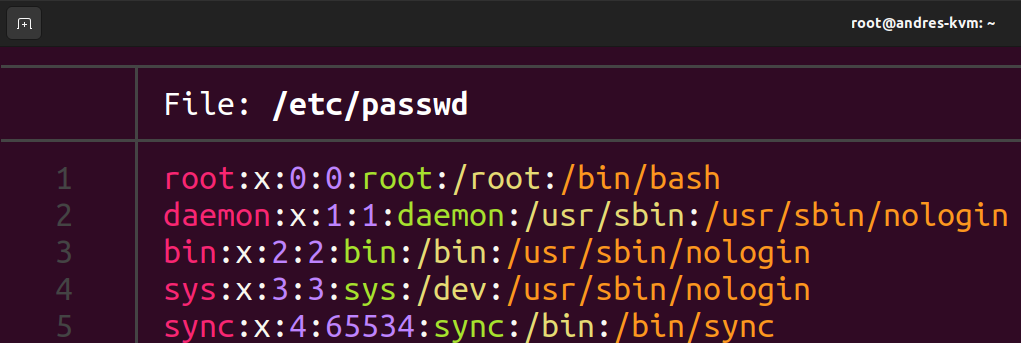
\includegraphics[width=\textwidth]{imagenes/passwdfile.png}
%    \caption{Ejemplo de entradas en el archivo.}
%\end{figure}

\addcontentsline{toc}{section}{Ejercicio 1}
\section*{Ejercicio 1}

Para ello voy a crear los siguientes programas:


\begin{figure}[H]
    \centering
    \begin{subfigure}{0.49\textwidth}
        \centering
        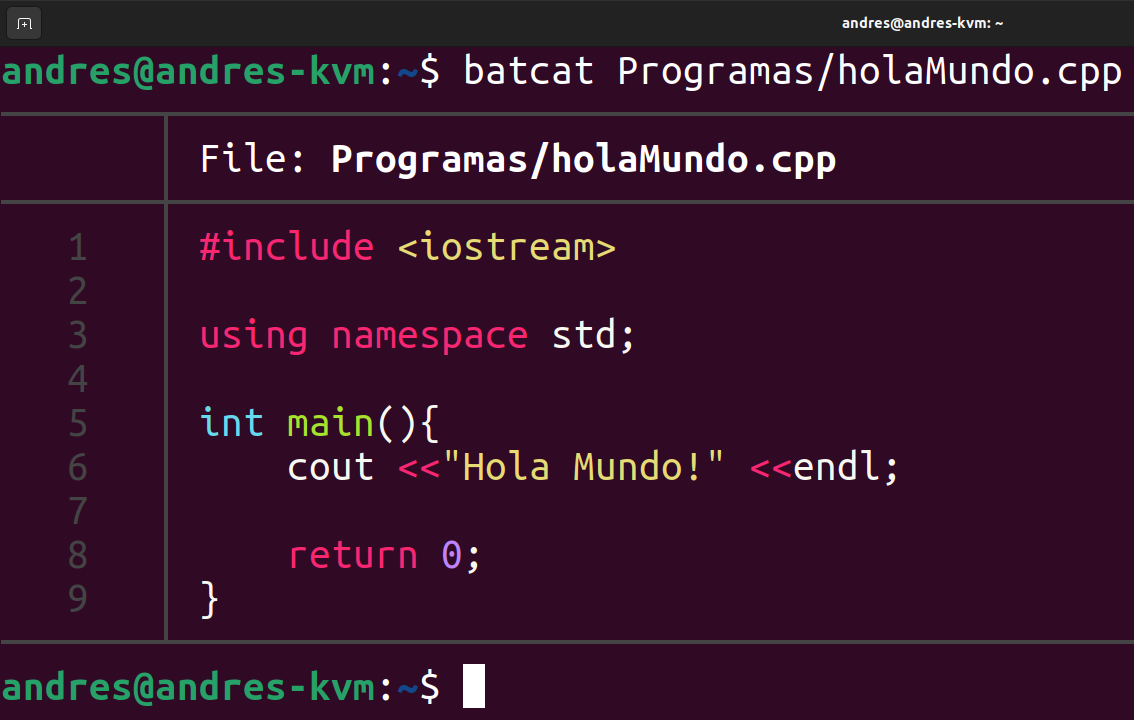
\includegraphics[width=\textwidth]{imagenes/Captura desde 2022-11-15 16-06-21.png}
        \caption{Versión C++.}
    \end{subfigure}
    \hfill
    \begin{subfigure}{0.49\textwidth}
        \centering
        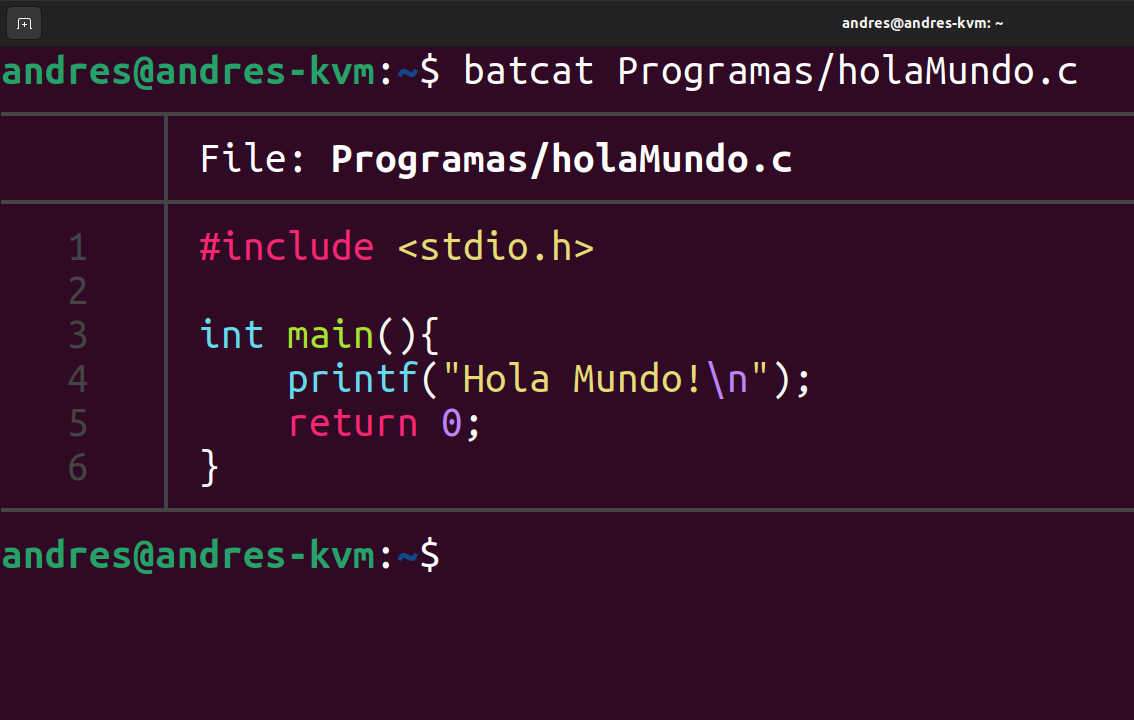
\includegraphics[width=\textwidth]{imagenes/Captura desde 2022-11-15 16-06-14.png}
        \caption{Versión C.}
    \end{subfigure}

    \caption{Distintas versiones del programa.}
\end{figure}



Y voy a usar las siguientes órdenes para compilarlos:

\bigskip

\verb|g++ -o salidaCPP holaMundo.cpp|

\verb|gcc -o salidaC holaMundo.c|

\bigskip

\addcontentsline{toc}{subsection}{Apartado A}
\subsection*{Apartado A}
A continuación explicaré que contiene cada sección, para obtener información se puede usar la orden \verb|man 5 elf|:

\begin{itemize}
    \item \textbf{.interp}: Esta sección almacena la ruta del intérprete del programa. Si el archivo tiene un segmento que incluye esta sección, los atributos de la sección tendrán el bit \texttt{SHF\_ALLOC}. La sección es de tipo \texttt{SHT\_PROGBITS}.
    
    \item \textbf{.got}: Esta sección almacena la tabla de desplazamientos global (Global Offset Table). Es de tipo \texttt{SH\_PROGBITS} y sus atributos son específicos del procesador. 
    
    \item \textbf{.got.plt}: Esta sección almacena la tabla de vinculación de procedimientos (Procedure Linkage Table). Es de tipo \texttt{SH\_PROGBITS} y sus atributos son específicos del procesador. Sirve para obtener las direcciones a funciones para posteriormente poder ser llamadas.
\end{itemize}

\newpage

\addcontentsline{toc}{subsection}{Apartado B}
\subsection*{Apartado B}

Ejecutando la orden \verb|readelf -S ejecutable| podemos obtener las secciones que componen el programa.

\begin{figure}[H]
    \centering
    \begin{subfigure}{0.49\textwidth}
        \centering
        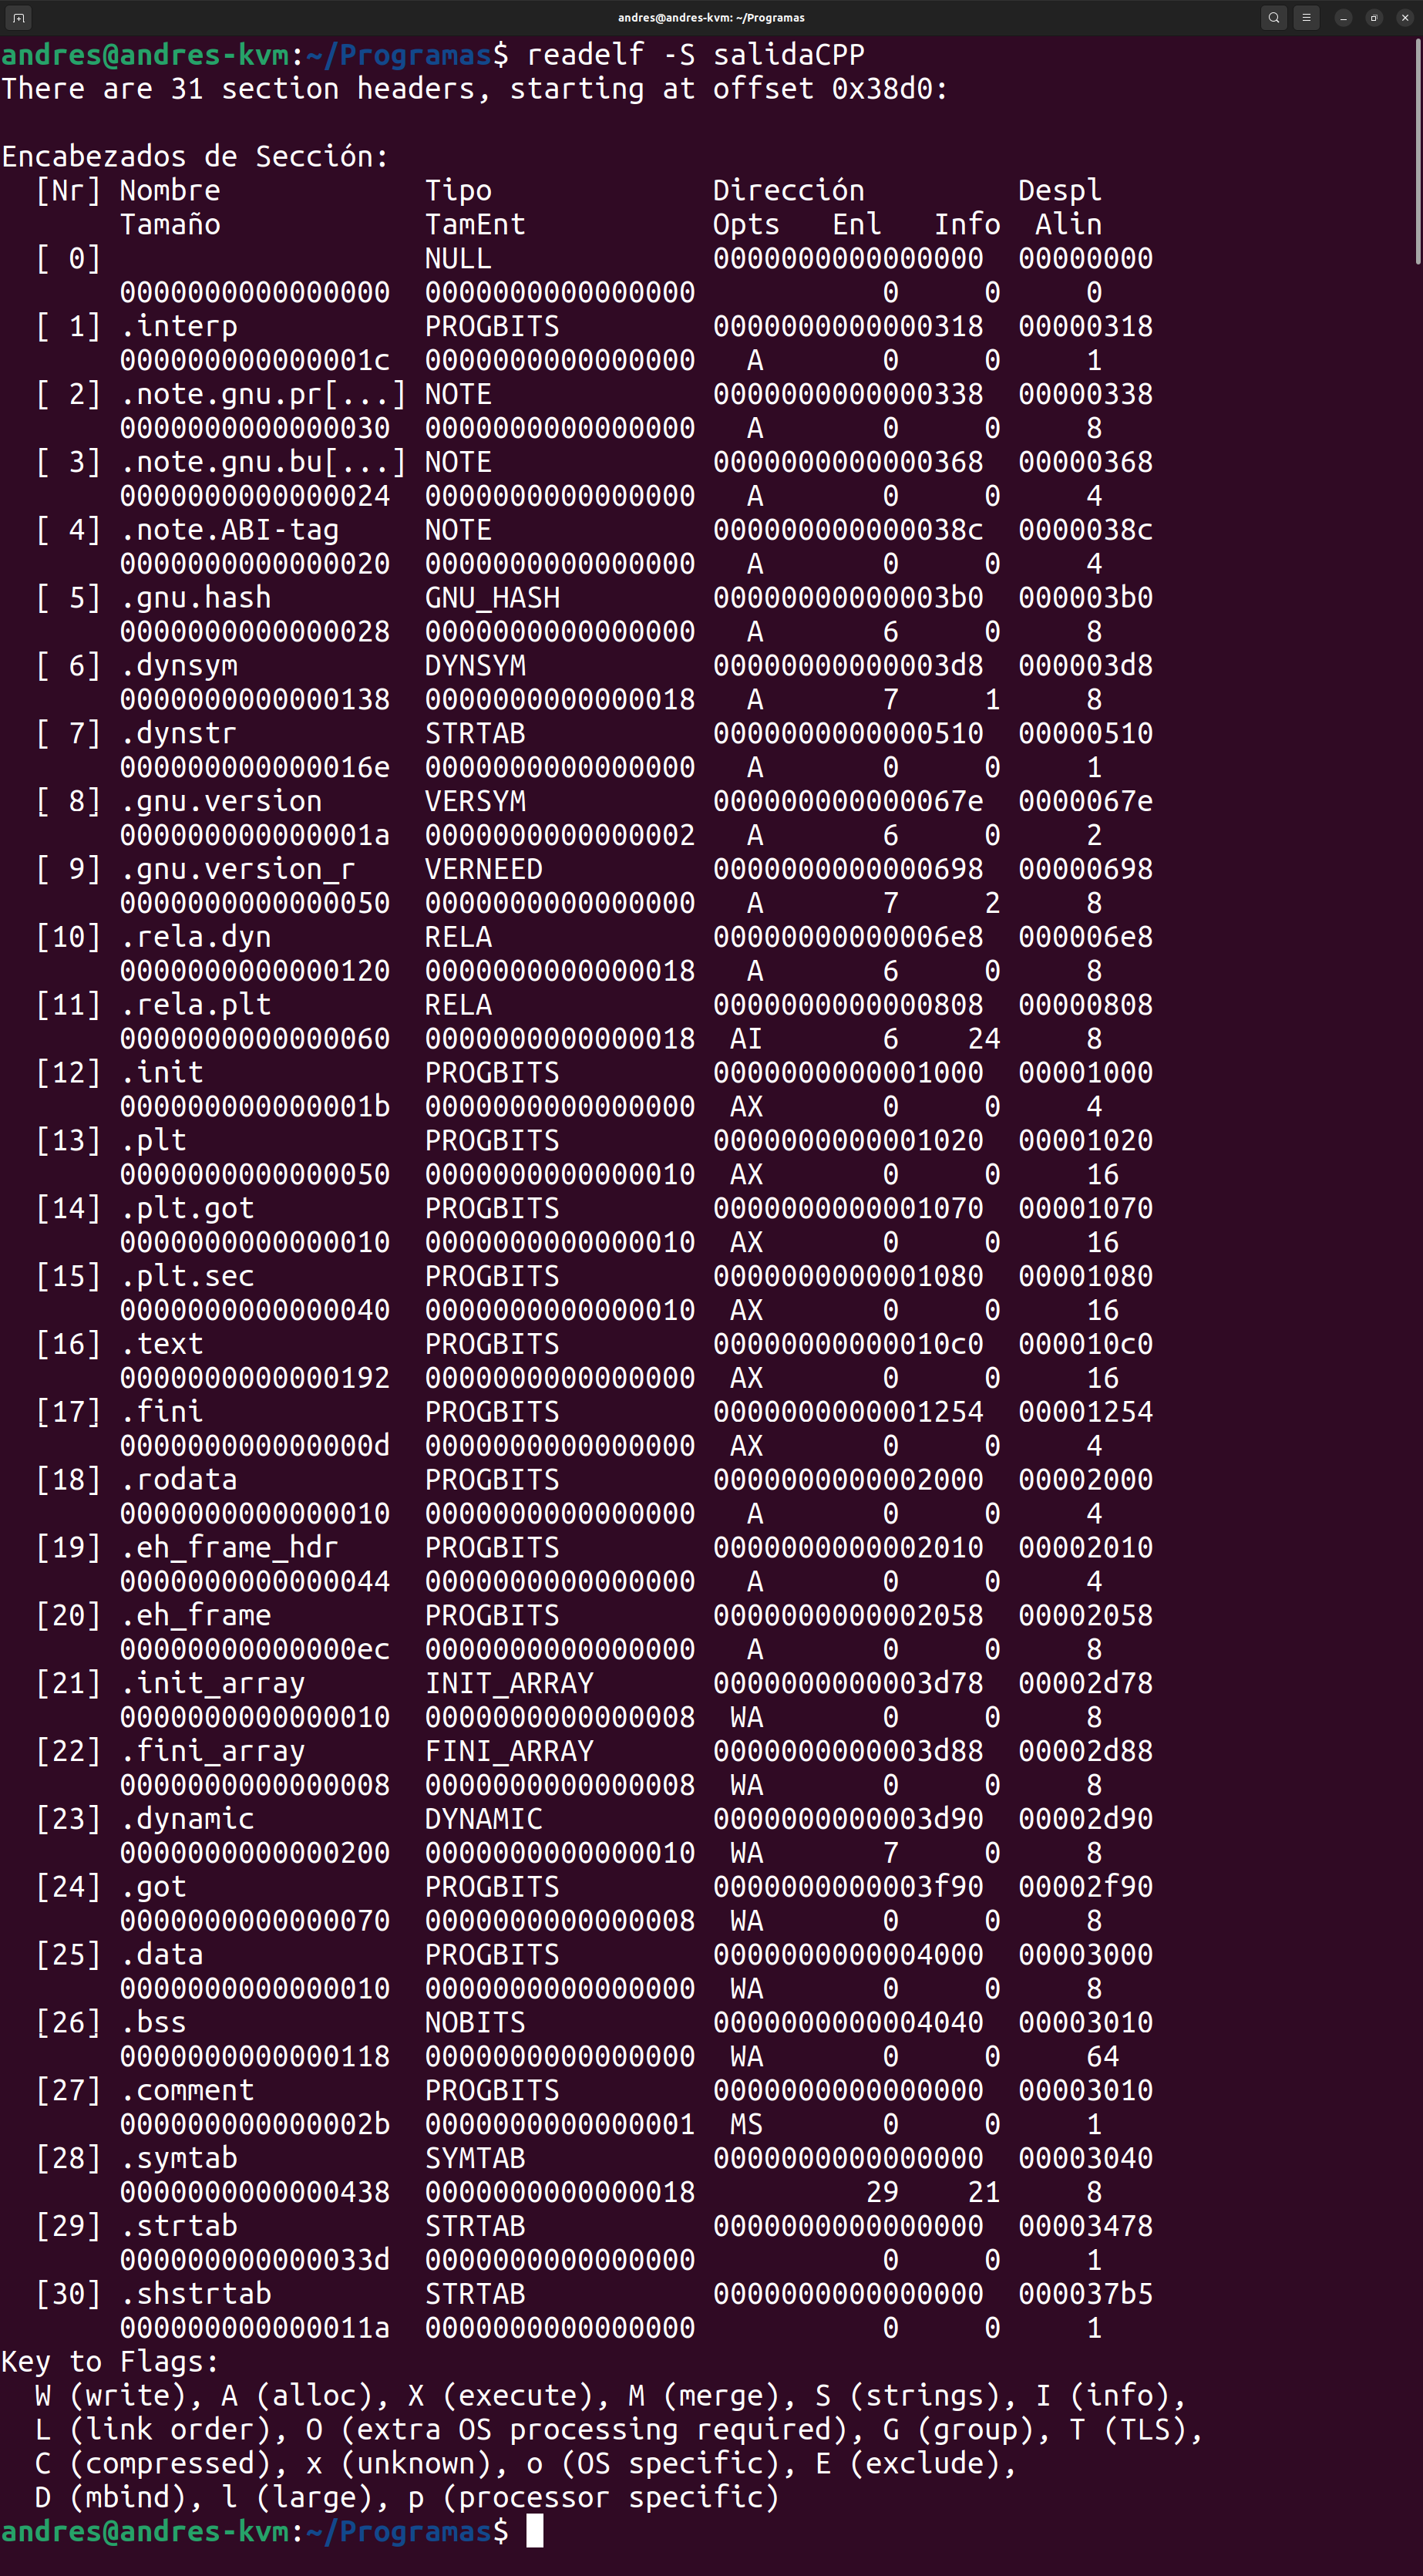
\includegraphics[width=\textwidth]{imagenes/CPP/merged.png}
        \caption{Versión C++.}
    \end{subfigure}
    \hfill
    \begin{subfigure}{0.49\textwidth}
        \centering
        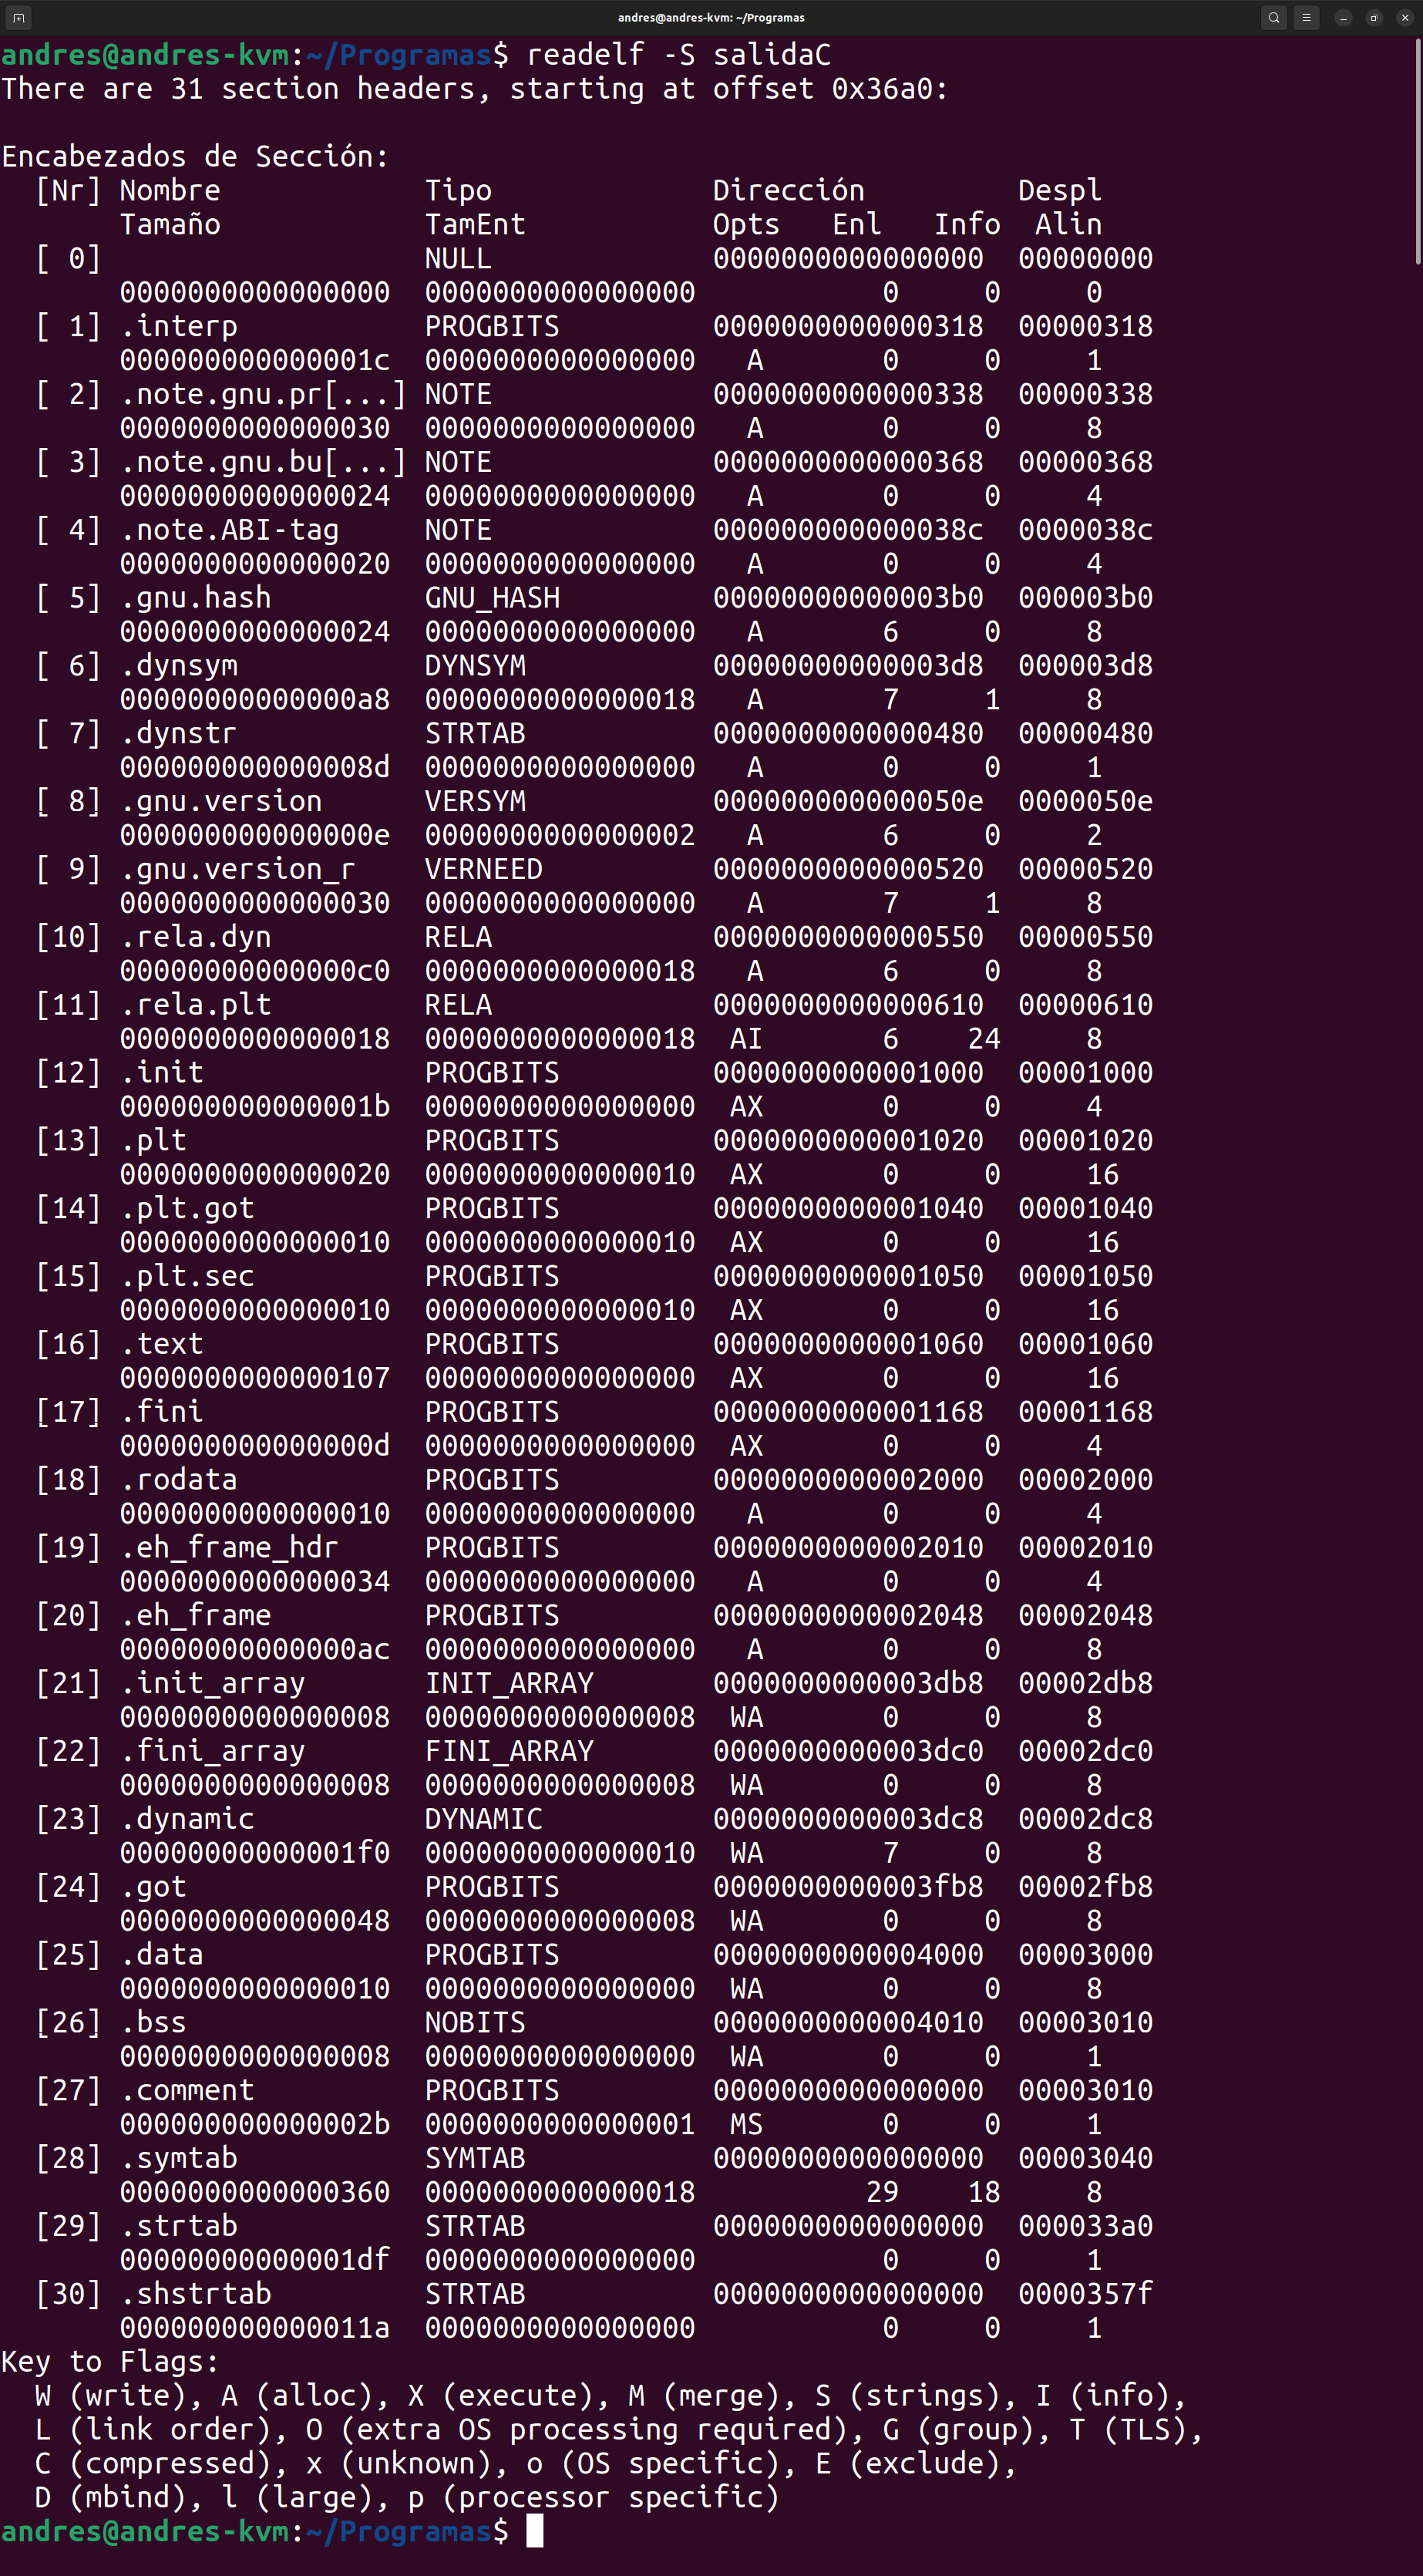
\includegraphics[width=\textwidth]{imagenes/C/merged.png}
        \caption{Versión C.}
    \end{subfigure}

    \caption{Secciones de los programas.}
\end{figure}

\newpage

Ahora, para mostrar por terminal la diferencia de los archivos a color se puede usar la orden \verb|icdiff archivo1 archivo2|.

%foto de icdiff (quizas haya que cortarlas)
\begin{figure}[H]
    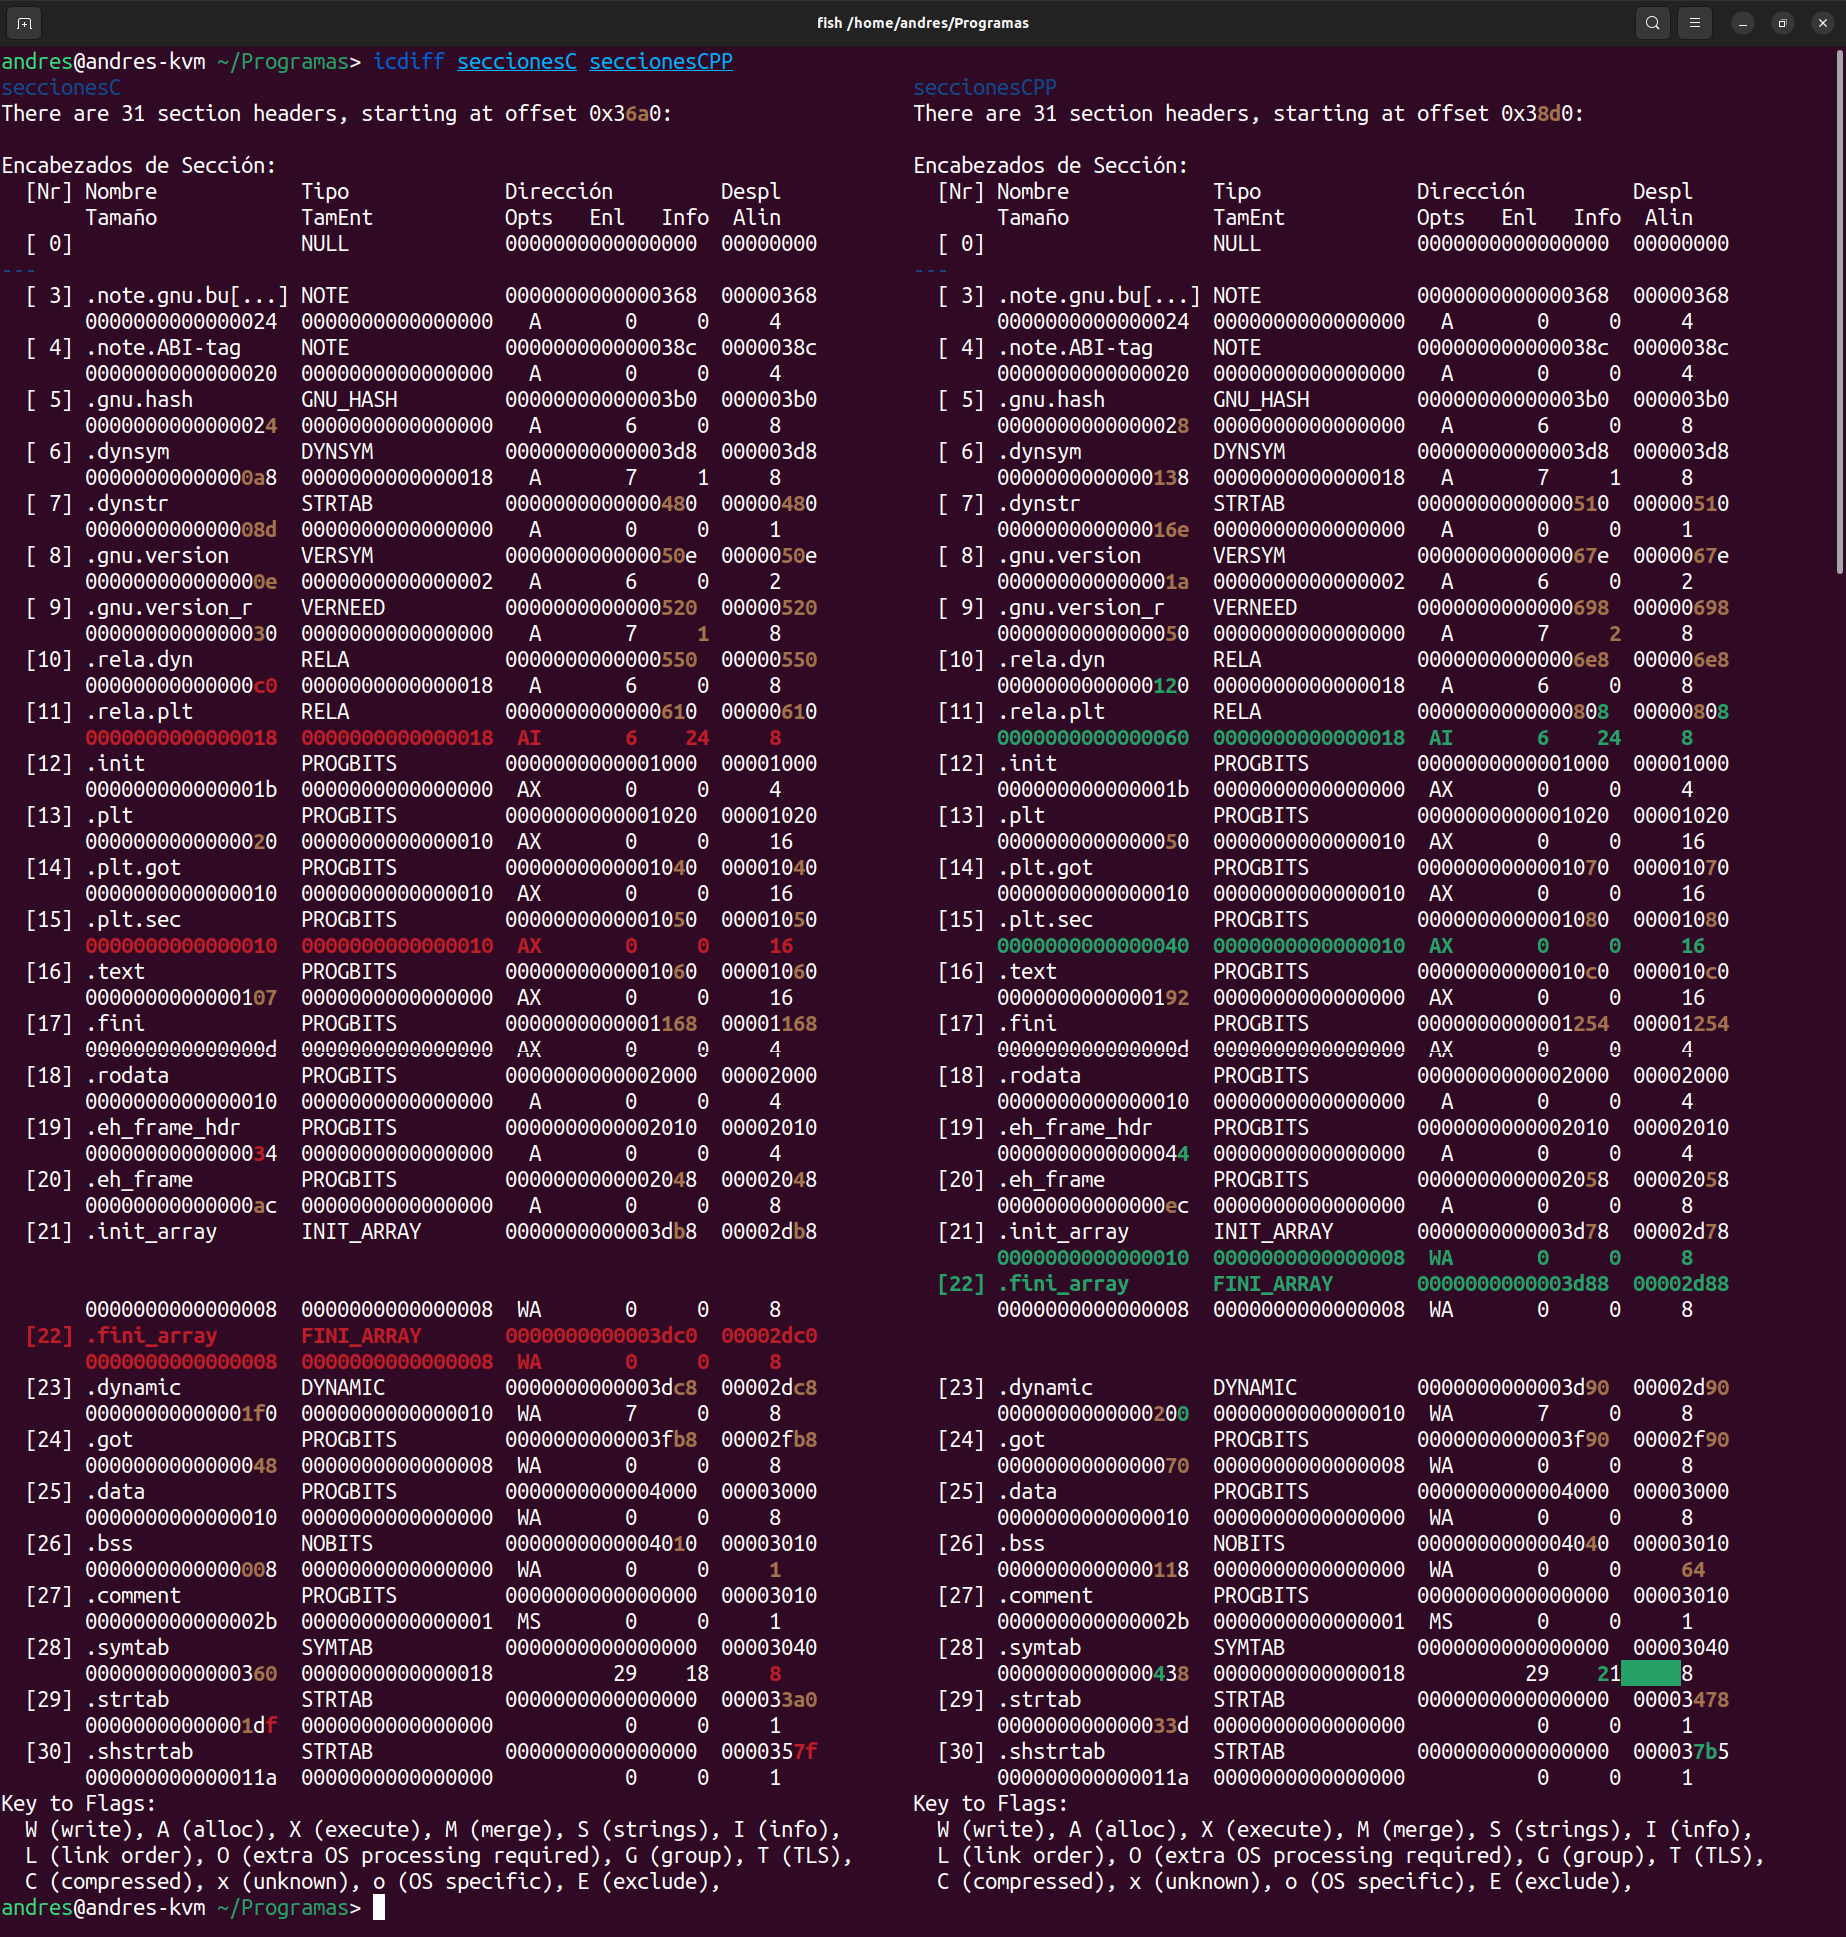
\includegraphics[width=\textwidth]{imagenes/icdiff/mergedicdiff.png}
    \caption{Diferencias entre ambas versiones compiladas.}
\end{figure}

Como se puede ver, en la primera línea, el offset es distinto, siendo más alto en el programa escrito en C++. Además, se puede ver que algunas secciones del programa escrito en C++ son ligeramente más grandes que la versión en C. Estas secciones son: \textbf{.gun.hash, .dynsym, .dynstr, .gun.version, .rela.dyn, .rela.plt, .plt, .plt.sec, .text, .eh\_frame\_hdr, .eh\_frame, .init\_array, .fini\_array, .dynamic, .got, .bss, .symtab, y .strtab.}

\bigskip

Por último, se puede ver que el desplazamiento (offset) y las direcciones de memoria de estas secciones varía entre una versión y otra.


\bigskip

Las secciones .ctors y .dtors contienen lo siguiente:

\begin{itemize}
    \item \textbf{.ctors}: Esta sección almacena punteros inicializados a las funciones del constructor de C++ (constructores de las clases).
    \item \textbf{.dtors}: Esta sección almacena punteros inicializados a las funciones del destructor de C++ (destructores de las clases).
\end{itemize}

\newpage

\addcontentsline{toc}{subsection}{Apartado C}
\subsection*{Apartado C}

Mediante la orden \verb|readelf -r programa| podemos ver las distintas secciones que contiene. Estas son:

\begin{itemize}
    \item \textbf{.rela.dyn}: Contiene las entradas de reubicación para símbolos dinámicos; es decir, estas variables deben ser reubicadas en tiempo de ejecución.
    \item \textbf{.rela.plt}: Contiene las entradas de reubicación para símbolos de funciones. Al igual que el anterior, deben ser reubicadas en tiempo de ejecución.
\end{itemize}

Además, la versión de C++ tiene más entradas que la versión de C, como pasó en el apartado anterior.

\bigskip

\addcontentsline{toc}{section}{Ejercicio 2}
\section*{Ejercicio 2}


\addcontentsline{toc}{subsection}{Apartado A}
\subsection*{Apartado A}

El comando \verb|objdump| tiene algunos switches similares a los de \verb|readelf|. A continuación voy a indicar algunos que se han usado en el ejercicio anterior:

\begin{itemize}
    \item \verb|readelf -r <archivo>| $\rightarrow$ \verb|objdump -Rr <archivo>|
    
    
    Muestra las entradas de reubicación del archivo ELF.

    %foto readelf y objdump side by side
    \begin{figure}[H]
        \centering
        \begin{subfigure}{0.49\textwidth}
            \centering
            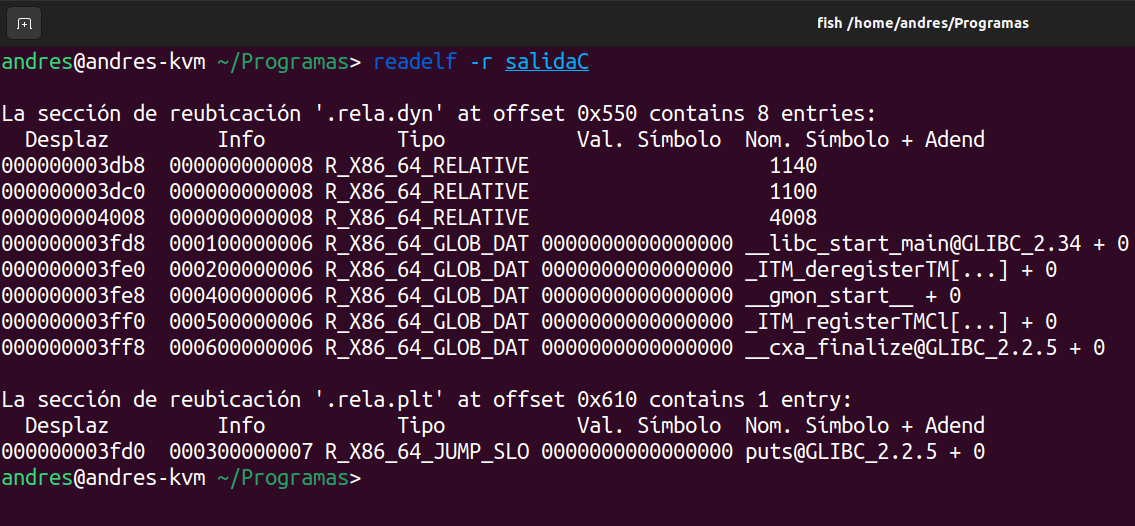
\includegraphics[width=\textwidth]{imagenes/Captura desde 2022-11-17 17-42-30.png}
        \end{subfigure}
        \hfill
        \begin{subfigure}{0.49\textwidth}
            \centering
            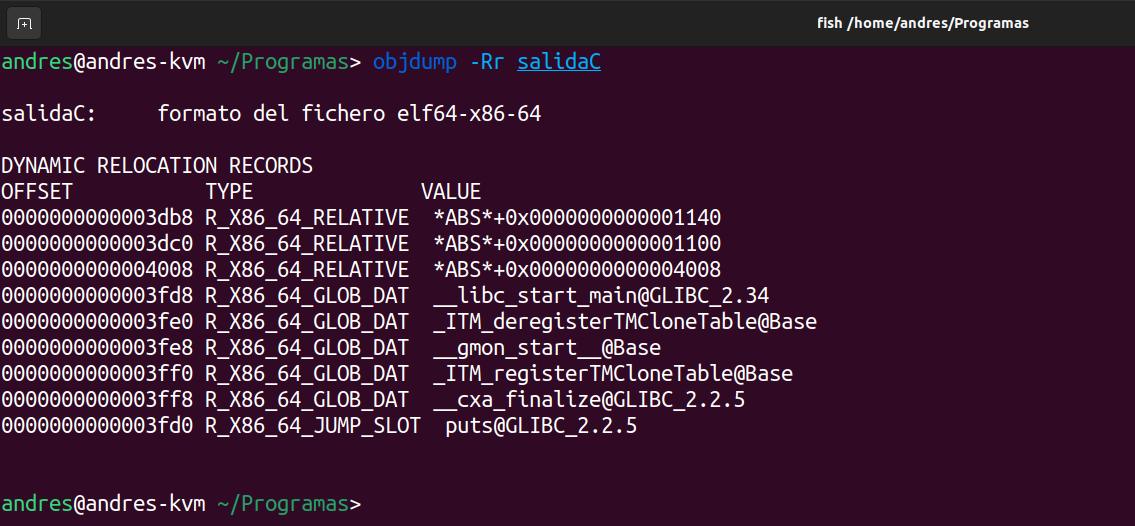
\includegraphics[width=\textwidth]{imagenes/Captura desde 2022-11-17 17-42-36.png}
        \end{subfigure}
    \end{figure}

    \item \verb|readelf -h <archivo>| $\rightarrow$ \verb|objdump -f <archivo>|
    
    Muestra las cabeceras del propio archivo ELF.

    %foto side by side
    \begin{figure}[H]
        \centering
        \begin{subfigure}{0.49\textwidth}
            \centering
            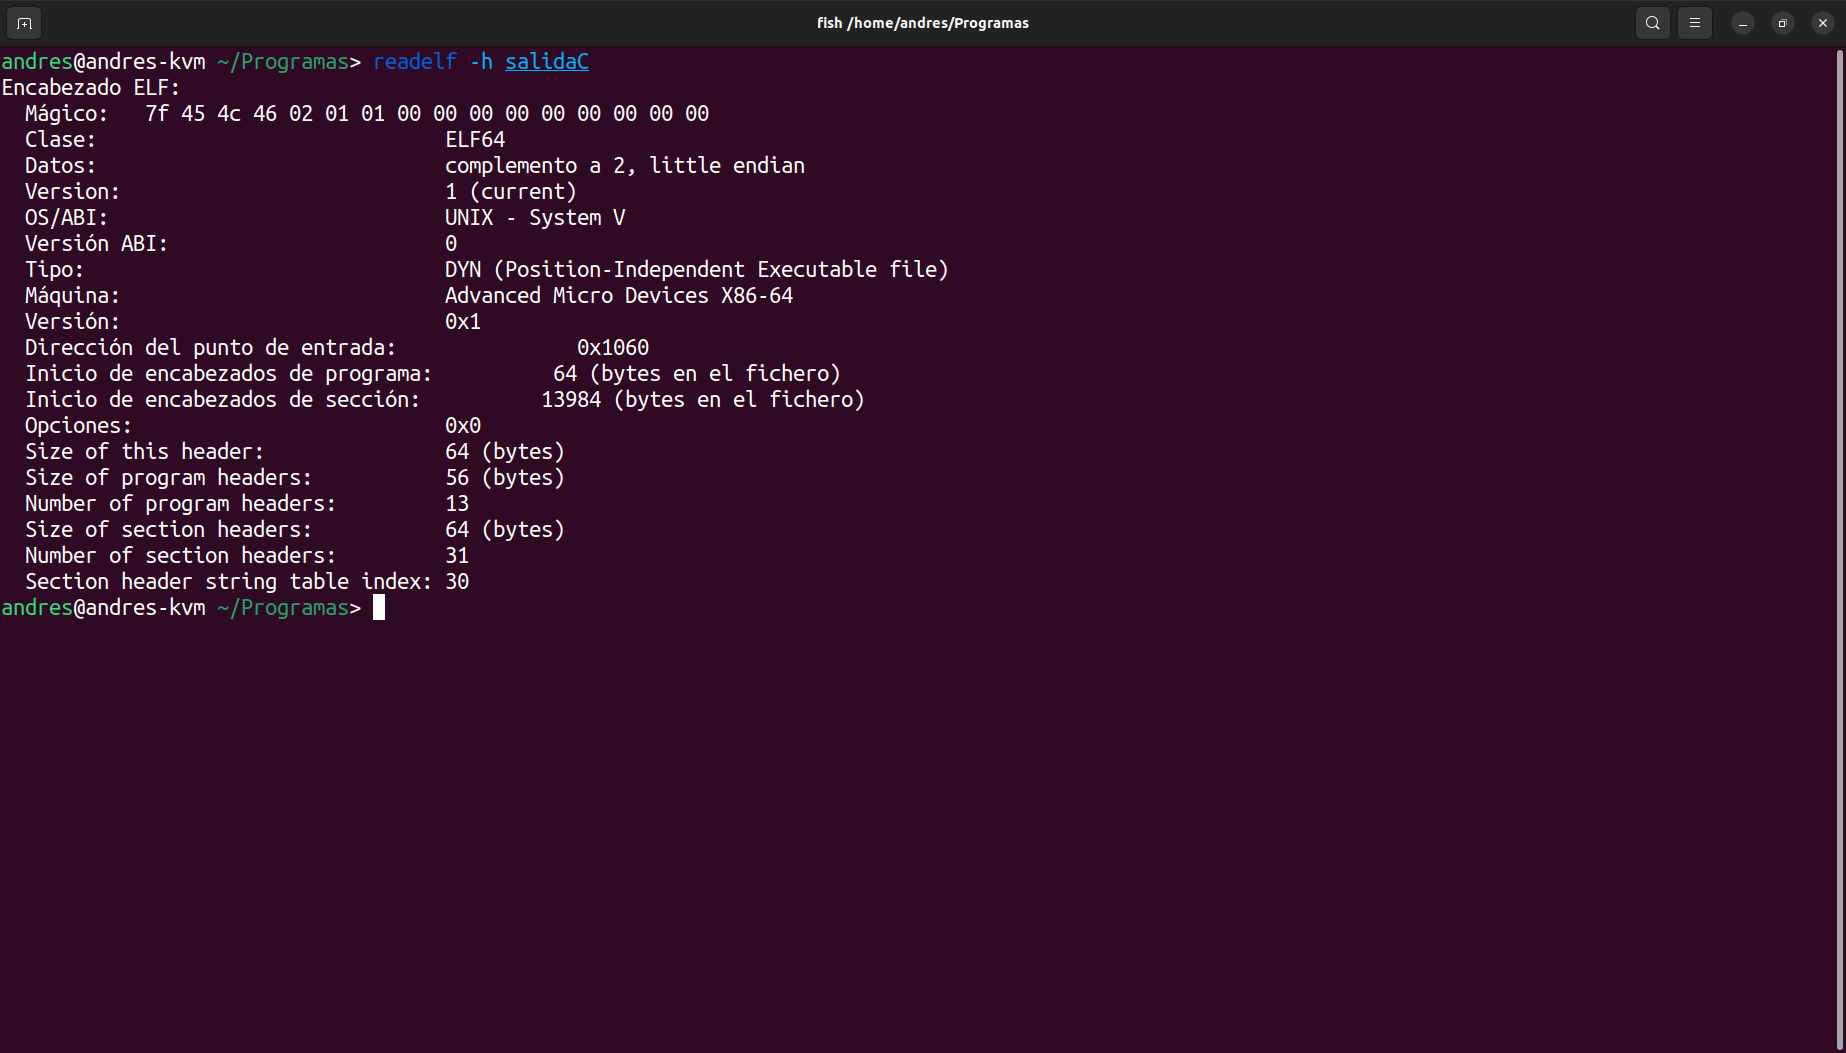
\includegraphics[width=\textwidth]{imagenes/Captura desde 2022-11-17 17-44-04.png}
        \end{subfigure}
        \hfill
        \begin{subfigure}{0.49\textwidth}
            \centering
            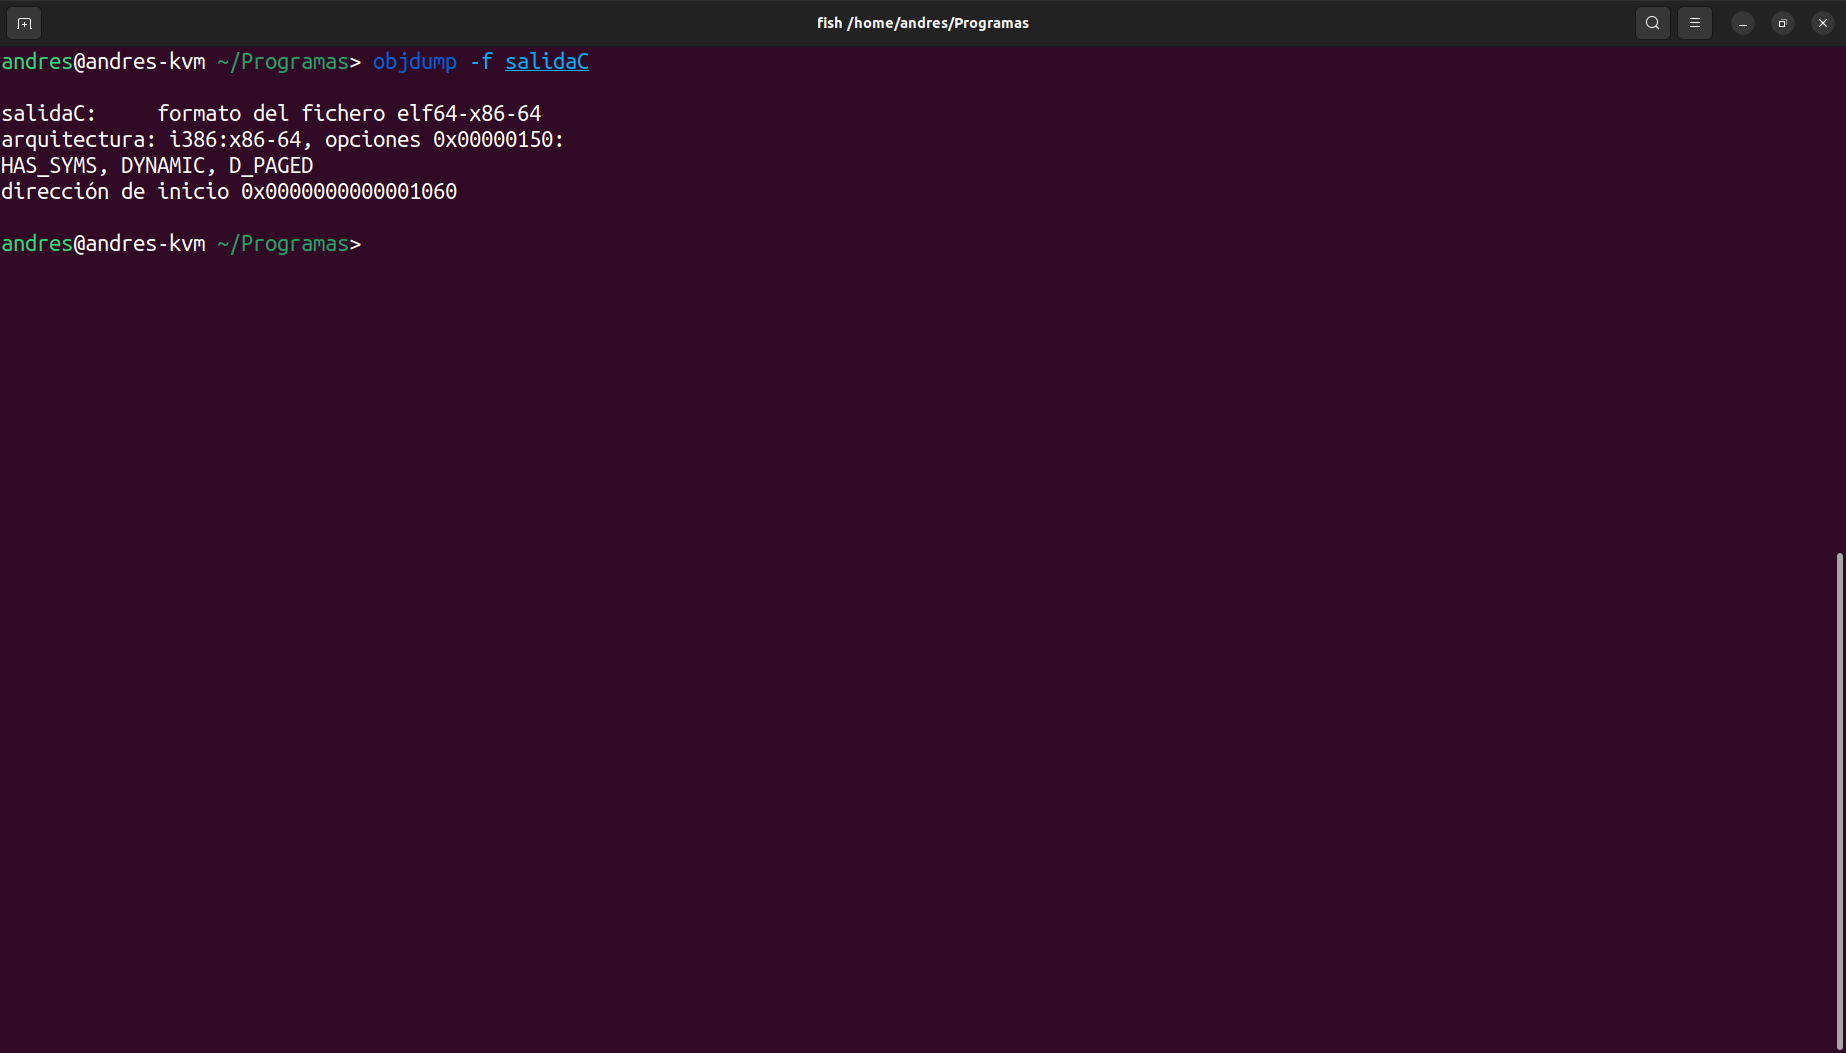
\includegraphics[width=\textwidth]{imagenes/Captura desde 2022-11-17 17-44-19.png}
        \end{subfigure}
    \end{figure}

    \newpage

    \item \verb|readelf -S <archivo>| $\rightarrow$ \verb|objdump -h <archivo>|
    
    Muestra la información de las cabeceras de sección (section headers).

    %foto side by side
    \begin{figure}[H]
        \centering
        \begin{subfigure}{0.49\textwidth}
            \centering
            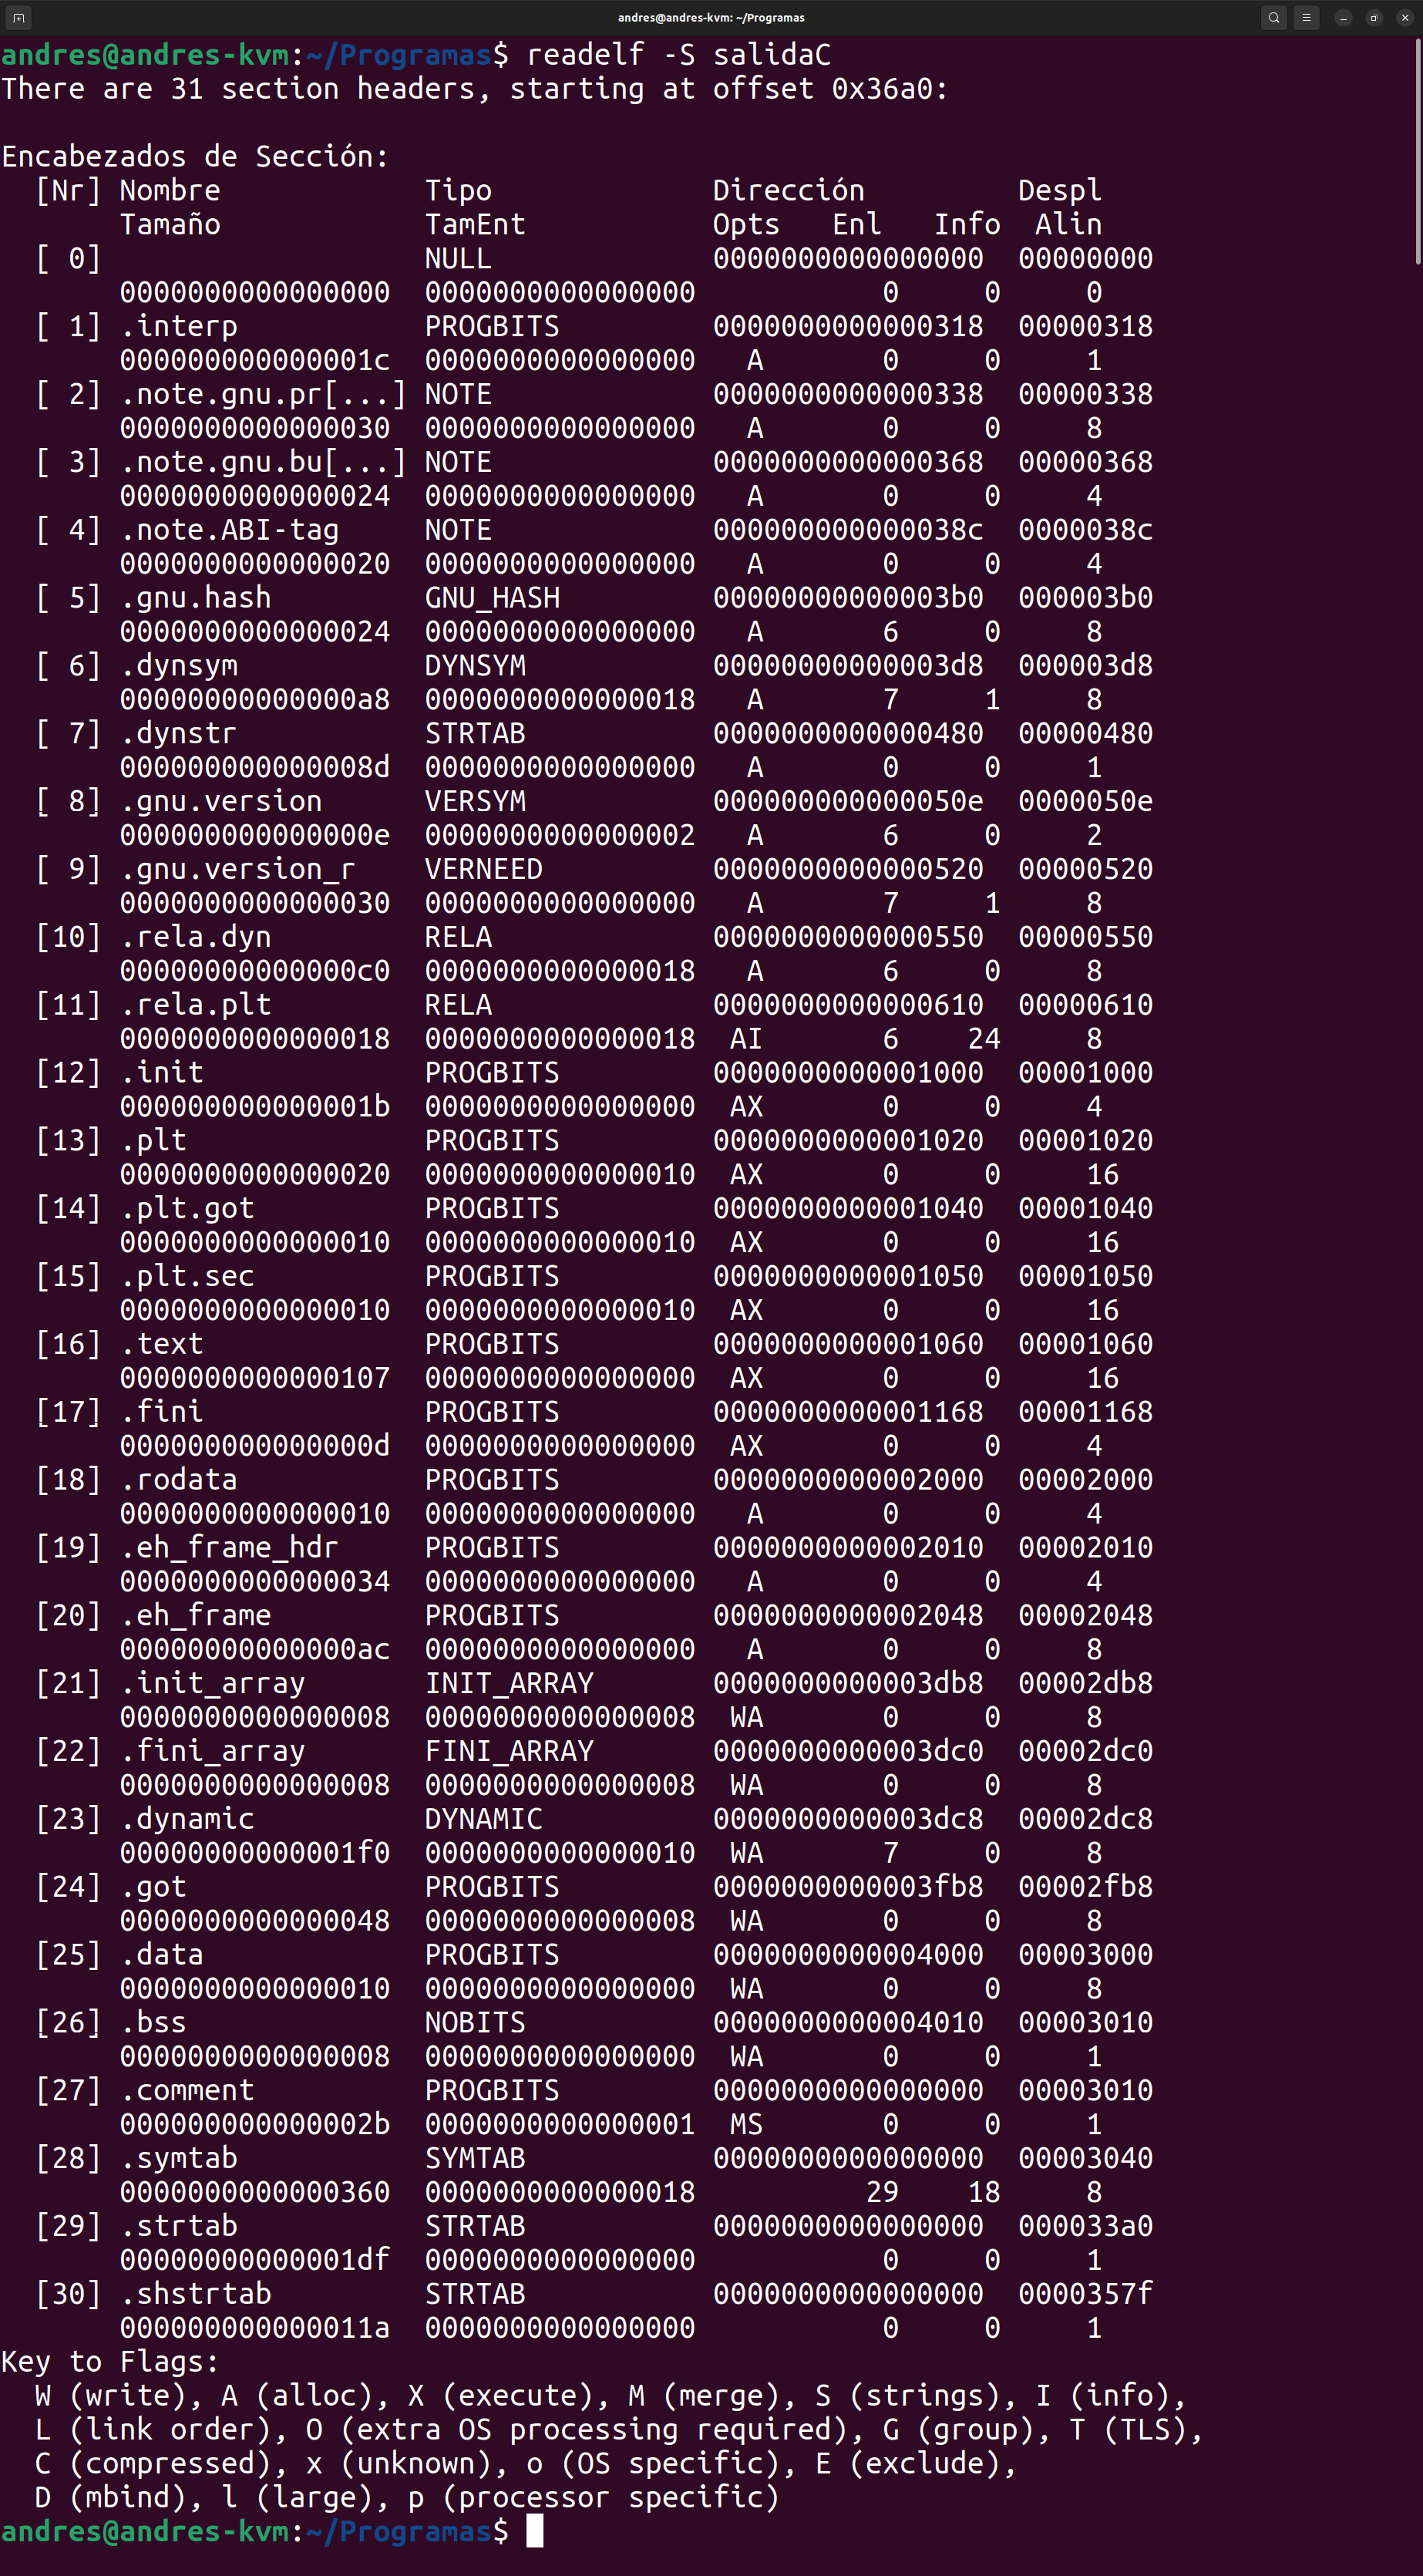
\includegraphics[width=\textwidth]{imagenes/C/merged.png}
        \end{subfigure}
        \hfill
        \begin{subfigure}{0.49\textwidth}
            \centering
            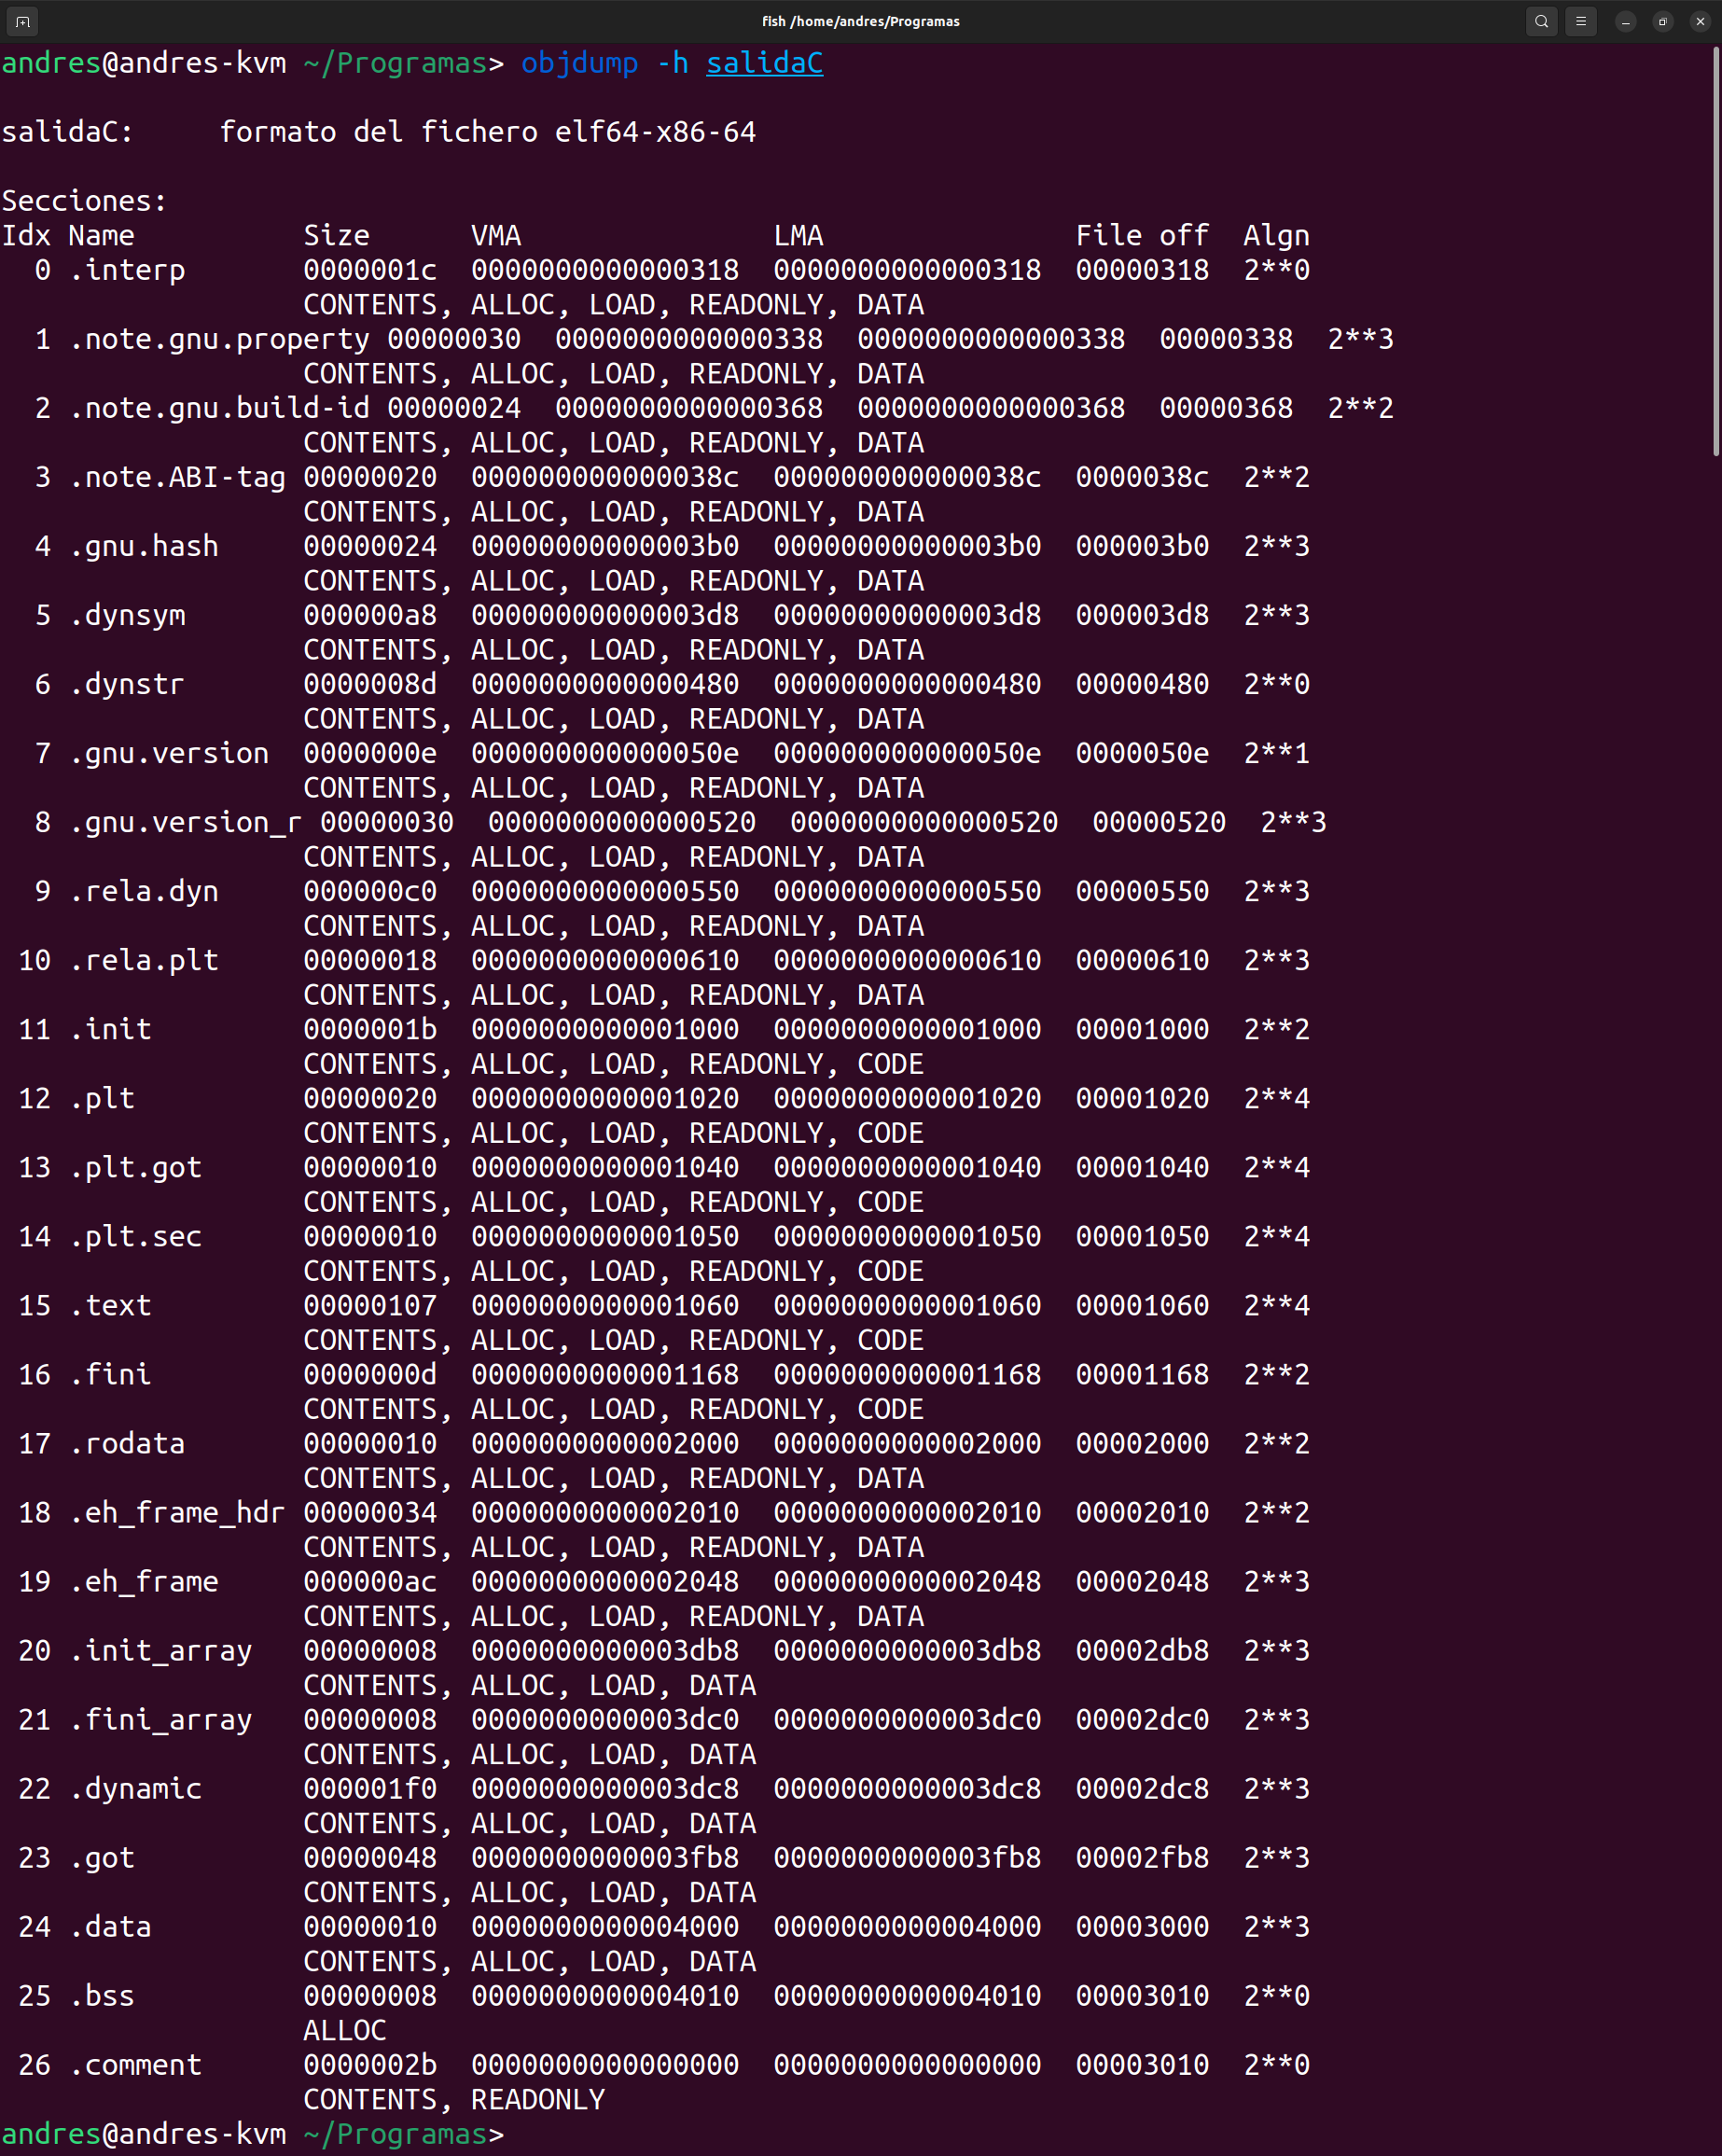
\includegraphics[width=\textwidth]{imagenes/merged.png}
        \end{subfigure}
    \end{figure}

    \newpage

    \item \verb|readelf -l <archivo>| $\rightarrow$ \verb|objdump -p <archivo>|
    
    Muestra las cabeceras del programa.

    %foto side by side
    \begin{figure}[H]
        \centering
        \begin{subfigure}{0.49\textwidth}
            \centering
            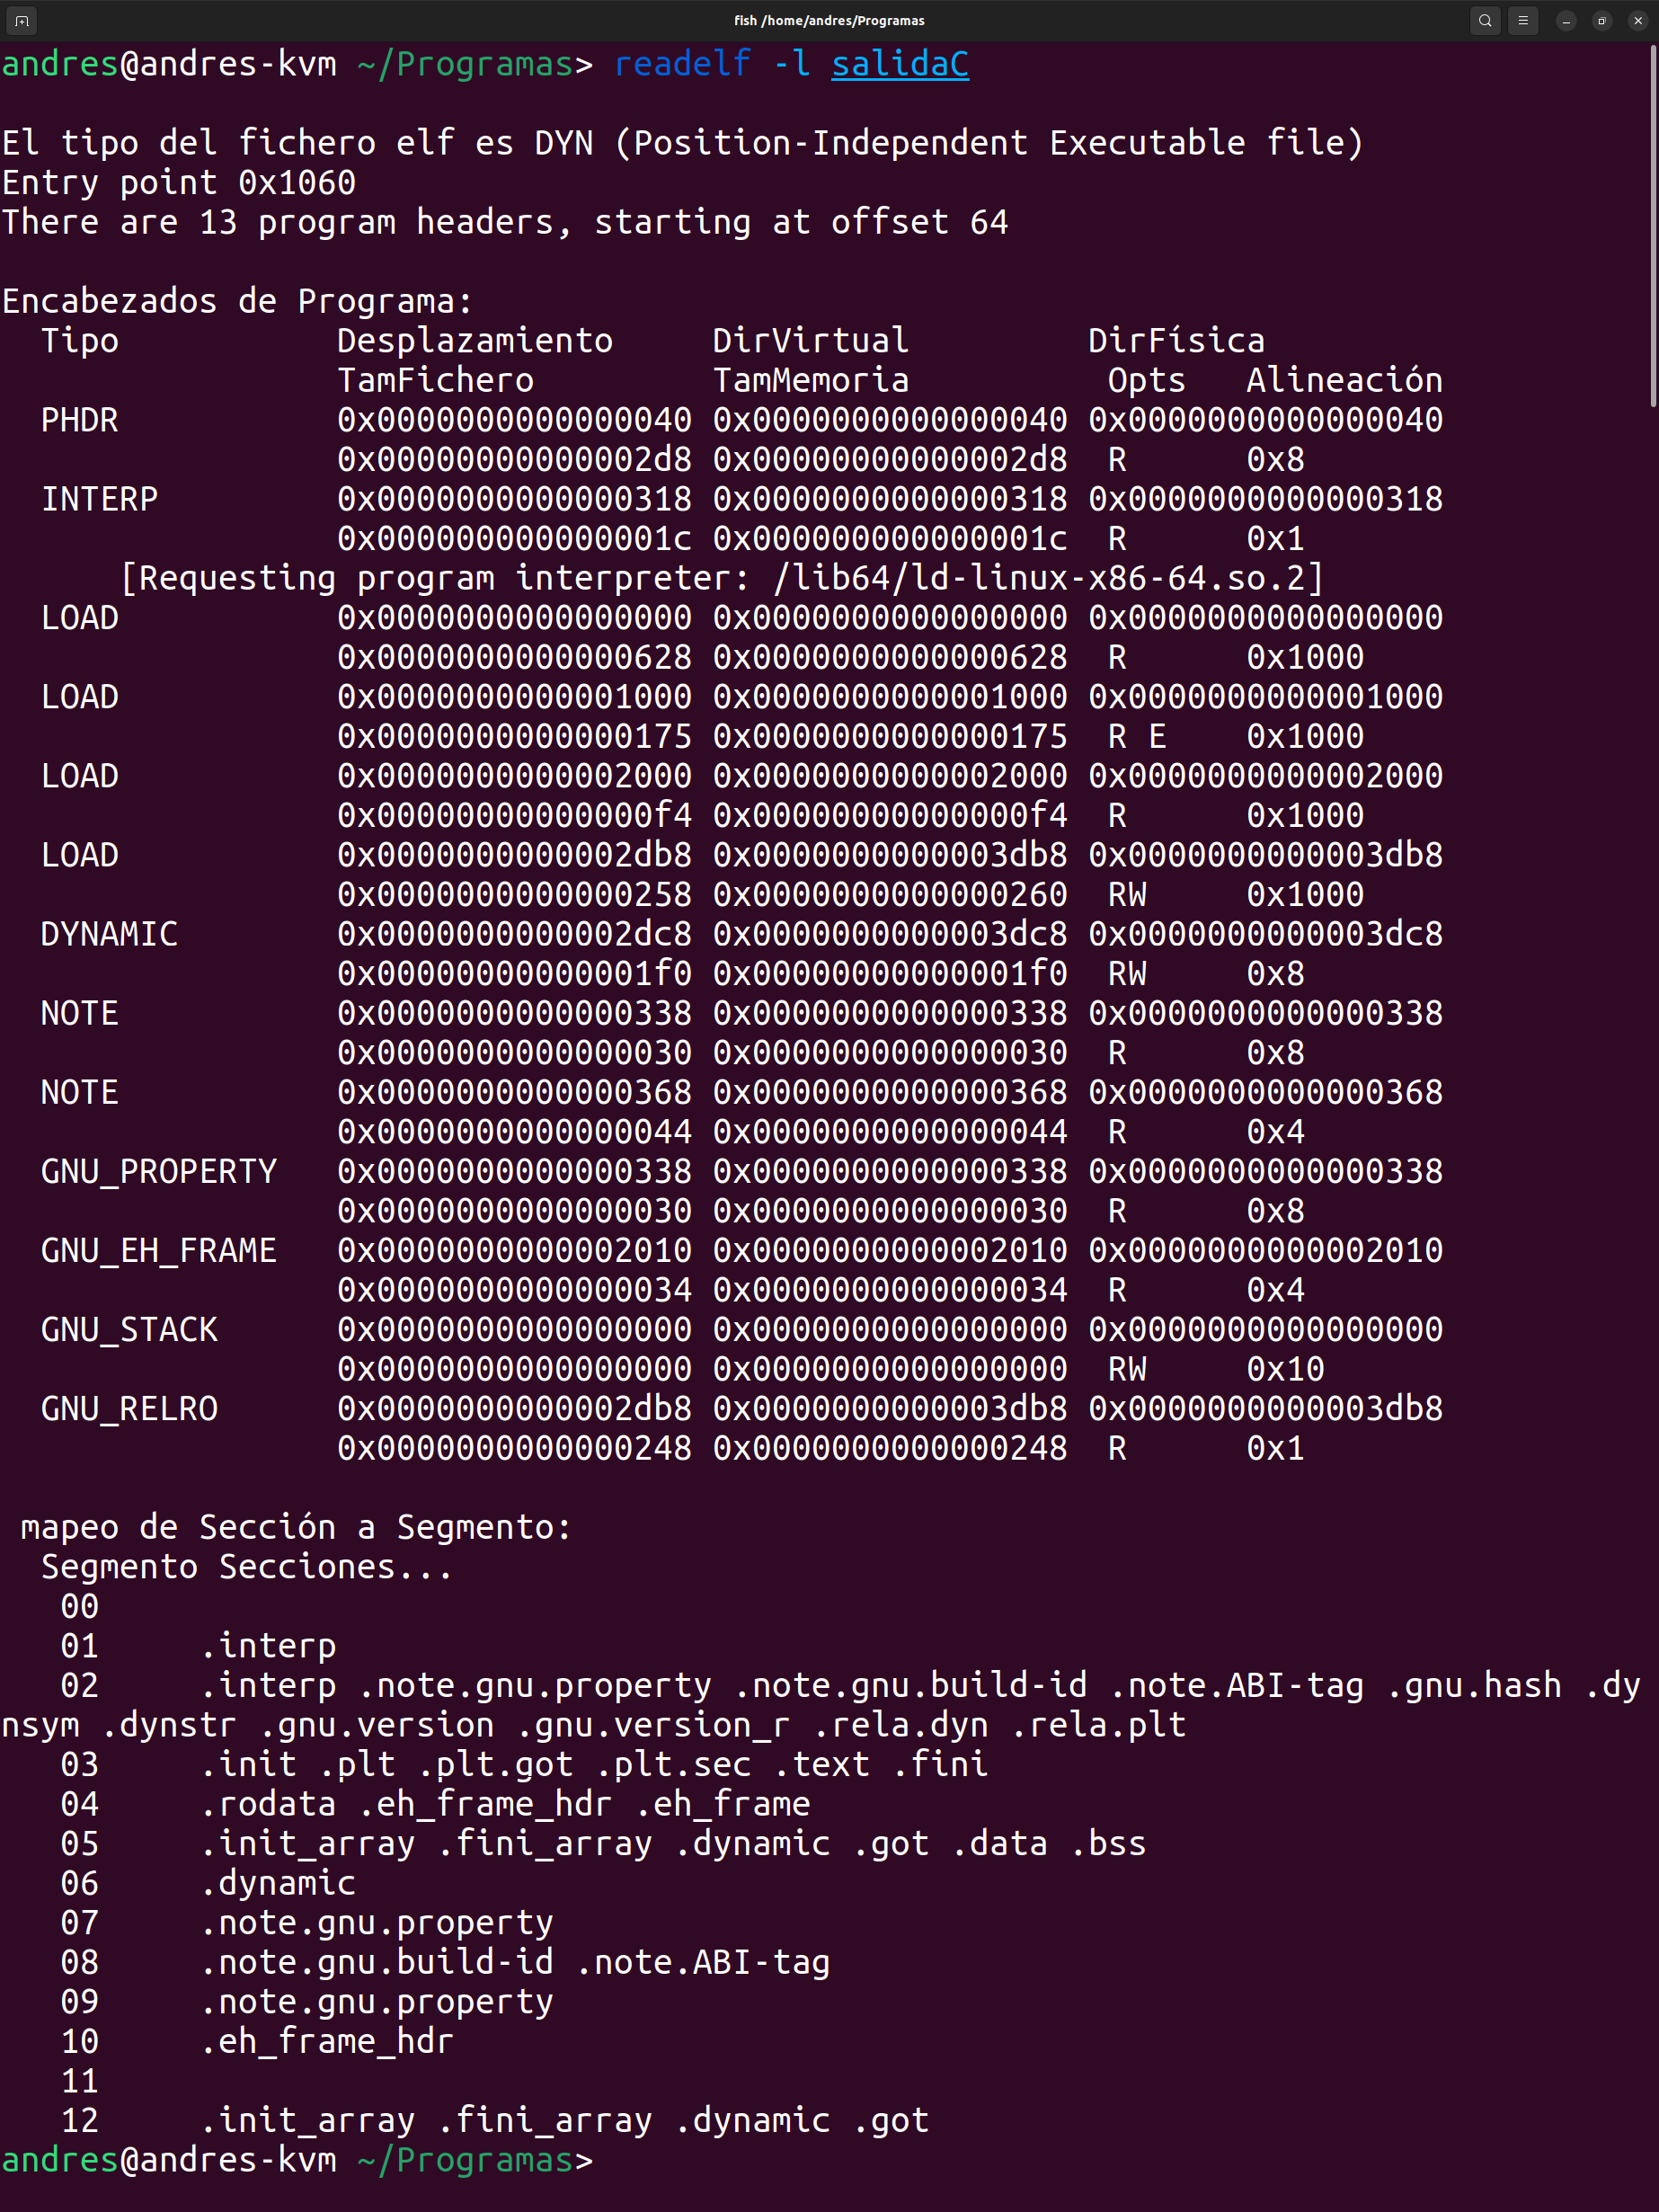
\includegraphics[width=\textwidth]{imagenes/mergedelfl.png}
        \end{subfigure}
        \hfill
        \begin{subfigure}{0.49\textwidth}
            \centering
            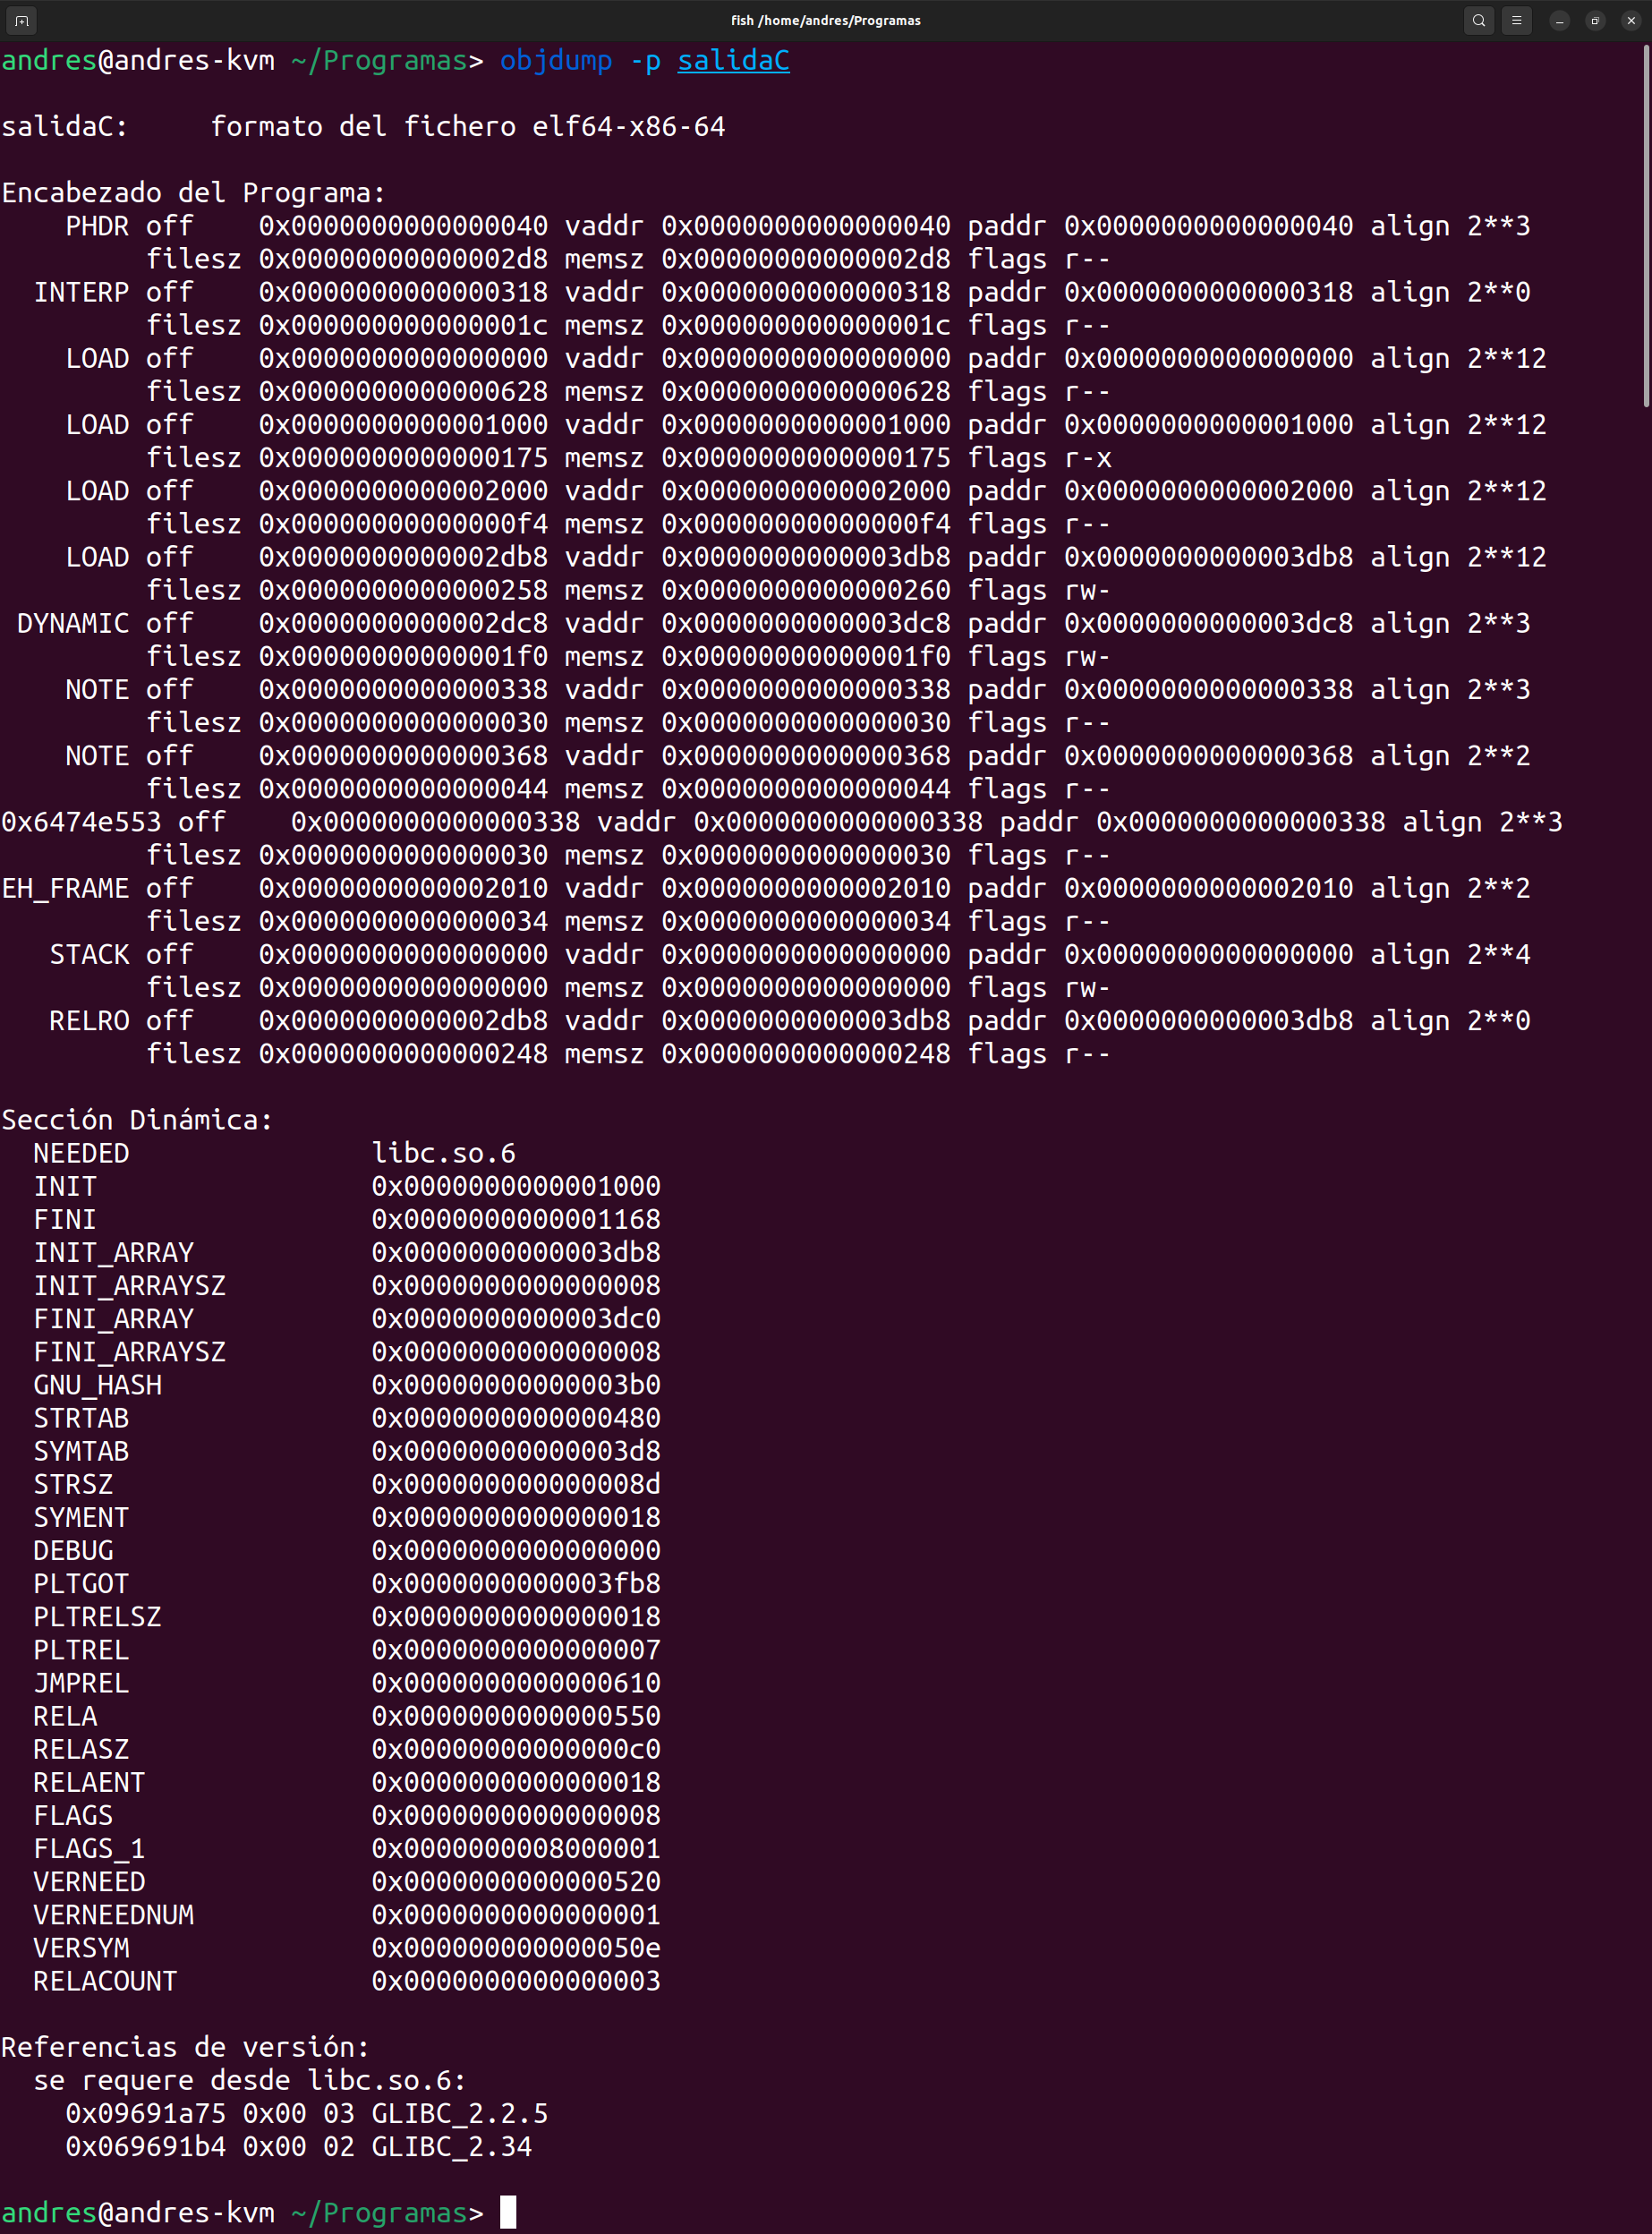
\includegraphics[width=\textwidth]{imagenes/mergedobjdumpp}
        \end{subfigure}
    \end{figure}    

\end{itemize}

% TABLE: READELF VS OBJDUMP
% -r / -Rr
% -h / -f
% -S / -h
% -l / -p

\addcontentsline{toc}{subsection}{Apartado B}
\subsection*{Apartado B}

Esta herramienta sirve de mucha utilidad desde el punto de ingeniería inversa, ya que permite el desensamblado de un ejecutable en las instrucciones máquina que lo compone.

%foto de eso
\begin{figure}[H]
    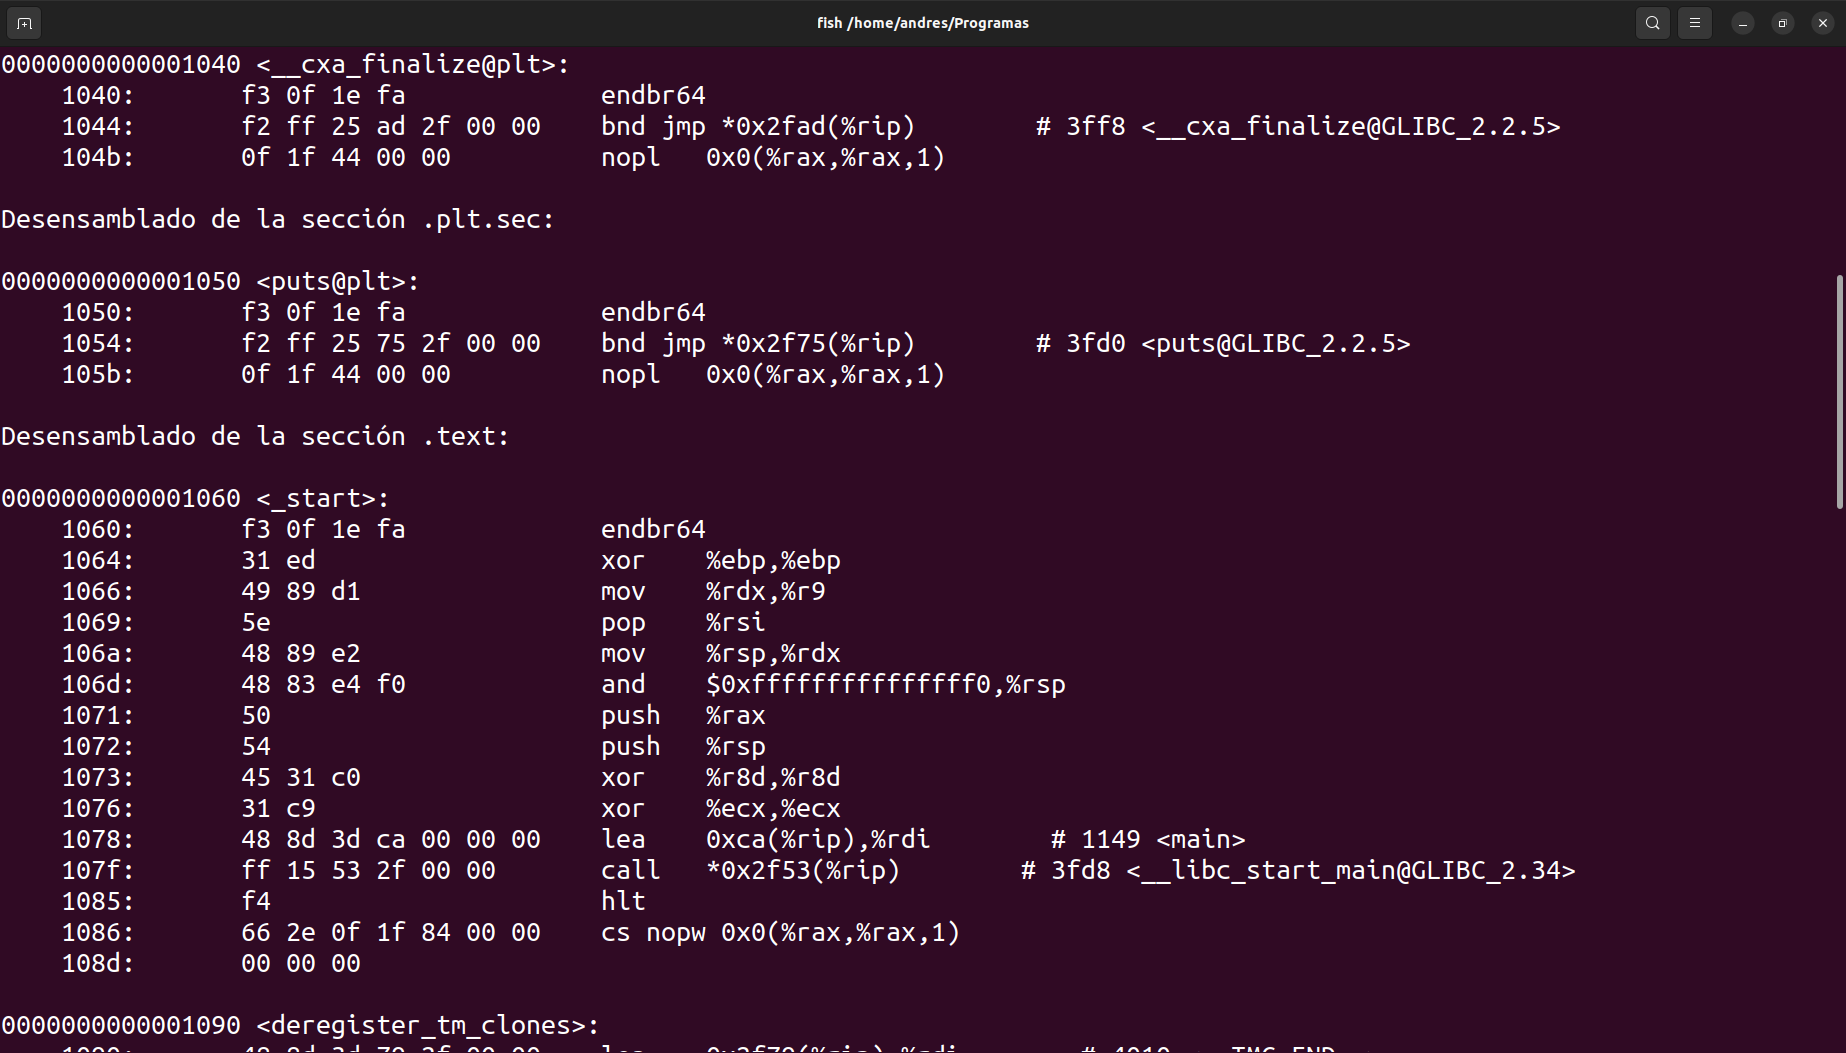
\includegraphics[width=\textwidth]{imagenes/Captura desde 2022-11-17 17-53-55.png}
    \caption{Salida producida por el comando \texttt{objdump -d salidaC}, se puede ver la llamada a \texttt{main} en \texttt{$<$\_start$>$}}
\end{figure}


\begin{figure}[H]
    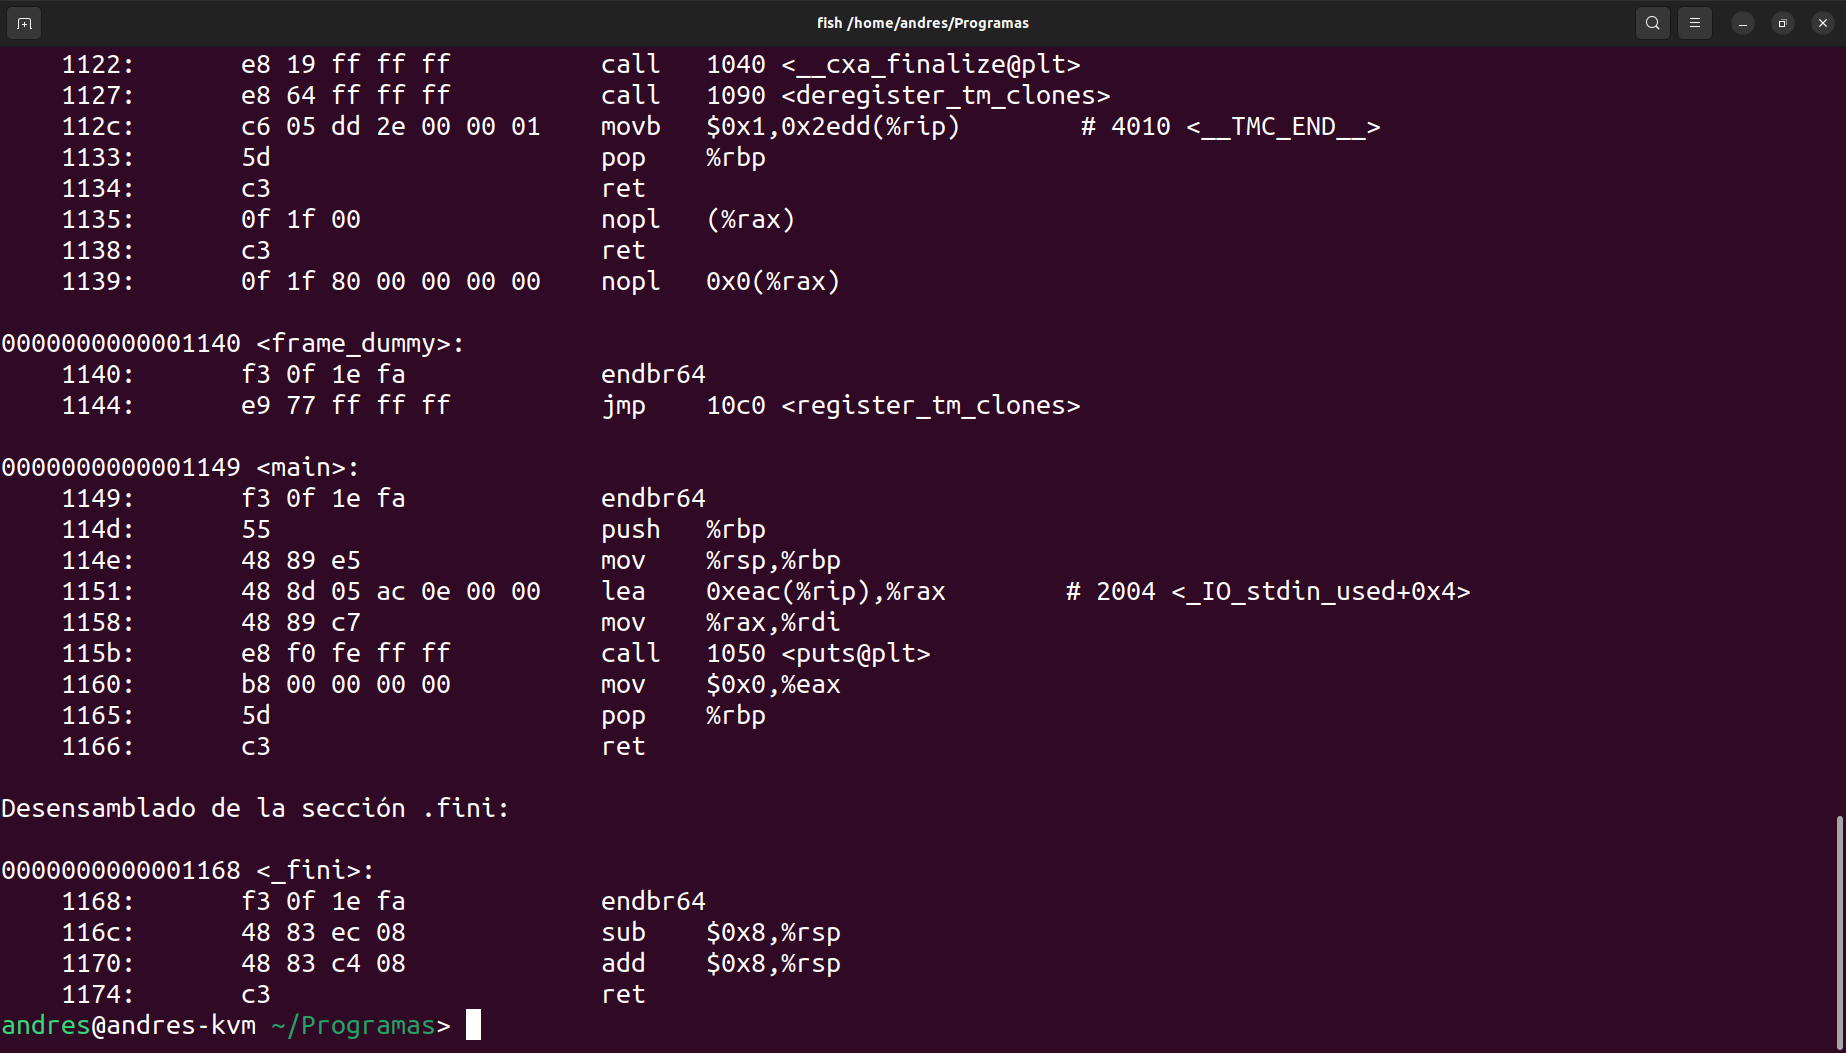
\includegraphics[width=\textwidth]{imagenes/Captura desde 2022-11-17 17-56-56.png}
    \caption{Función \texttt{$<$main$>$} compilada a de C a ensamblador.}
\end{figure}

Esto simplifica mucho el trabajo, ya que no es necesario buscar en los manuales de los procesadores que instrucción tiene cada código. Además, esto permite buscar vulnerabilidades en el programa o incluso el estudio de las distintas condiciones para que continúe el código para luego poder intentar saltarse las medidas de seguridad.

\bigskip

\addcontentsline{toc}{section}{Ejercicio 3}
\section*{Ejercicio 3}

He realizado la siguiente modificación al programa en su versión C:

%modificacion del rpograma con sleep
\begin{figure}[H]
    \centering
    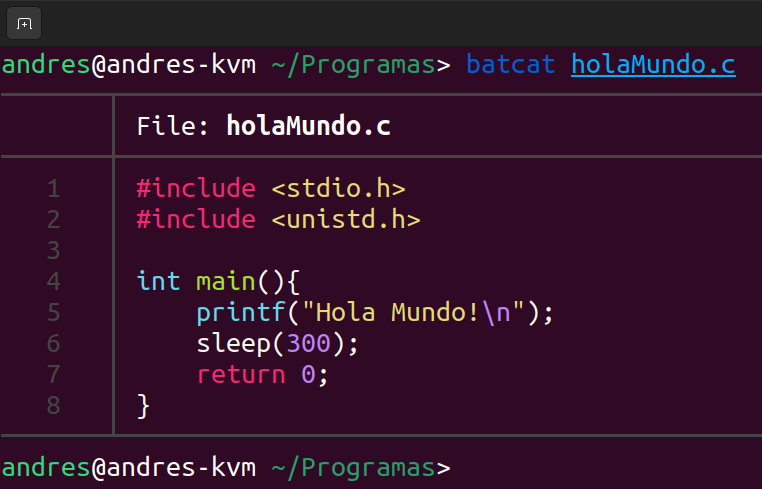
\includegraphics[width=0.7\textwidth]{imagenes/Captura desde 2022-11-17 18-12-25.png}
\end{figure}

Ahora, mediante el símbolo ``\&'' se puede ejecutar el programa en segundo plano. A continuación, se busca el proceso pasando la salida de la orden \verb|ps -e| mediante un pipe a la orden \verb|grep|. Por tanto, en mi caso, la orden para encontrar el PID del programa sería así: \texttt{ps -e $\vert$ grep hola}.

%salida de ps
\begin{figure}[H]
    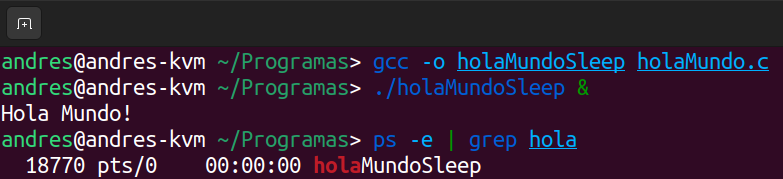
\includegraphics[width=\textwidth]{imagenes/ps.png}
\end{figure}

Y sabiendo que tiene el PID \textbf{18770}, con cualquier orden para mostrar texto como \texttt{nano, cat, bat} se puede ver lo que contiene.

%salida de proc pid maps
\begin{figure}[H]
    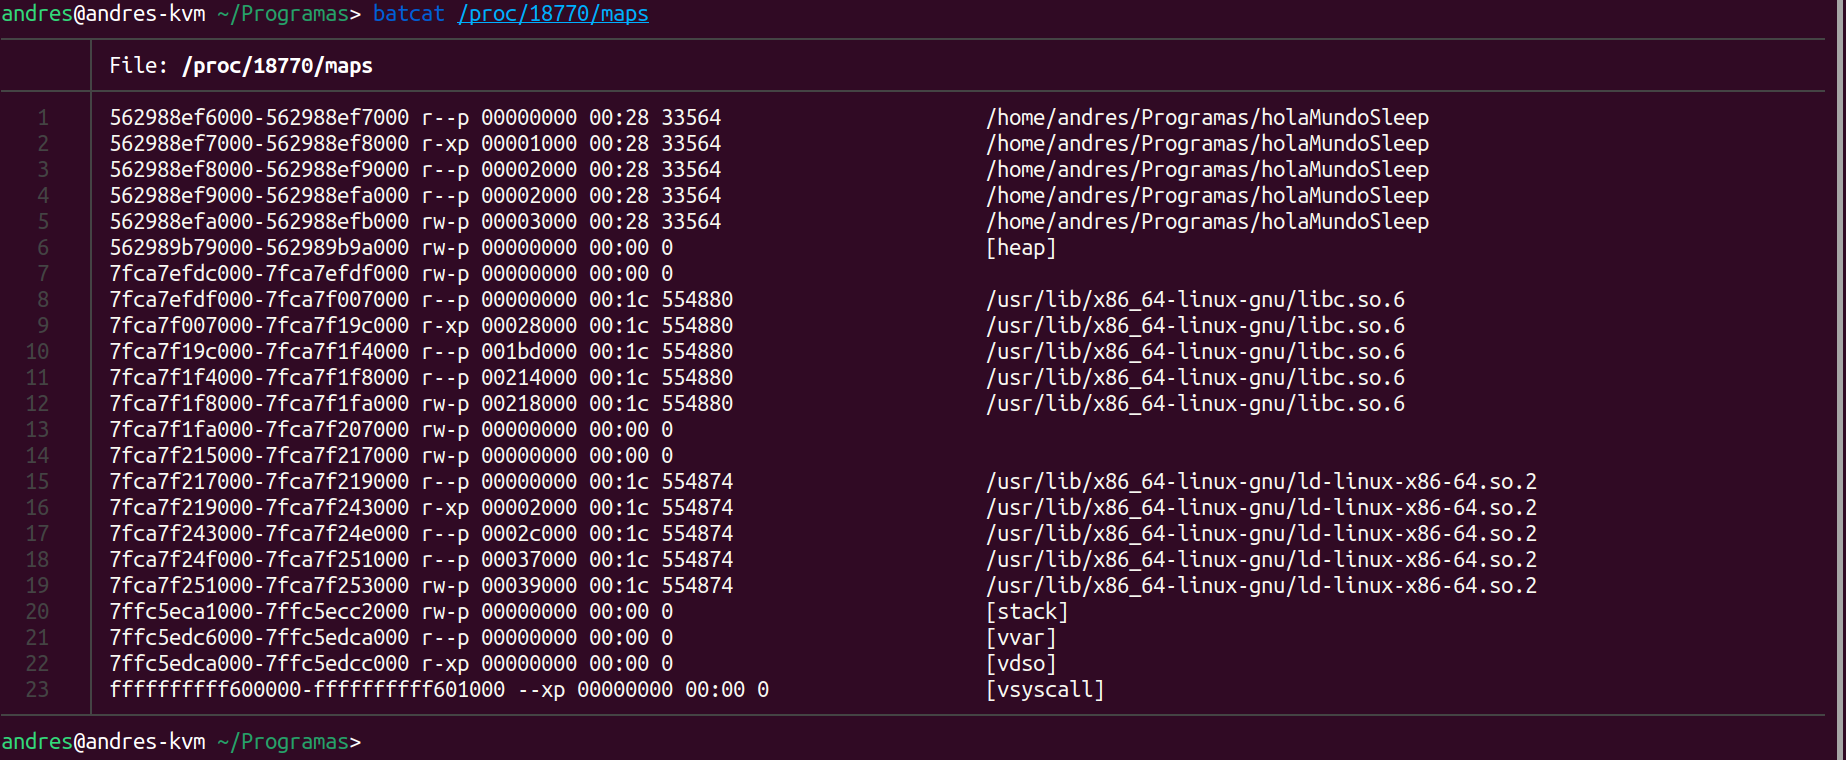
\includegraphics[width=\textwidth]{imagenes/procPID.png}
\end{figure}

Ahora, con la orden \verb|readelf -S <archivo>| podemos ver las secciones que componen el ejecutable:

%foto de la salida
\begin{figure}[H]
    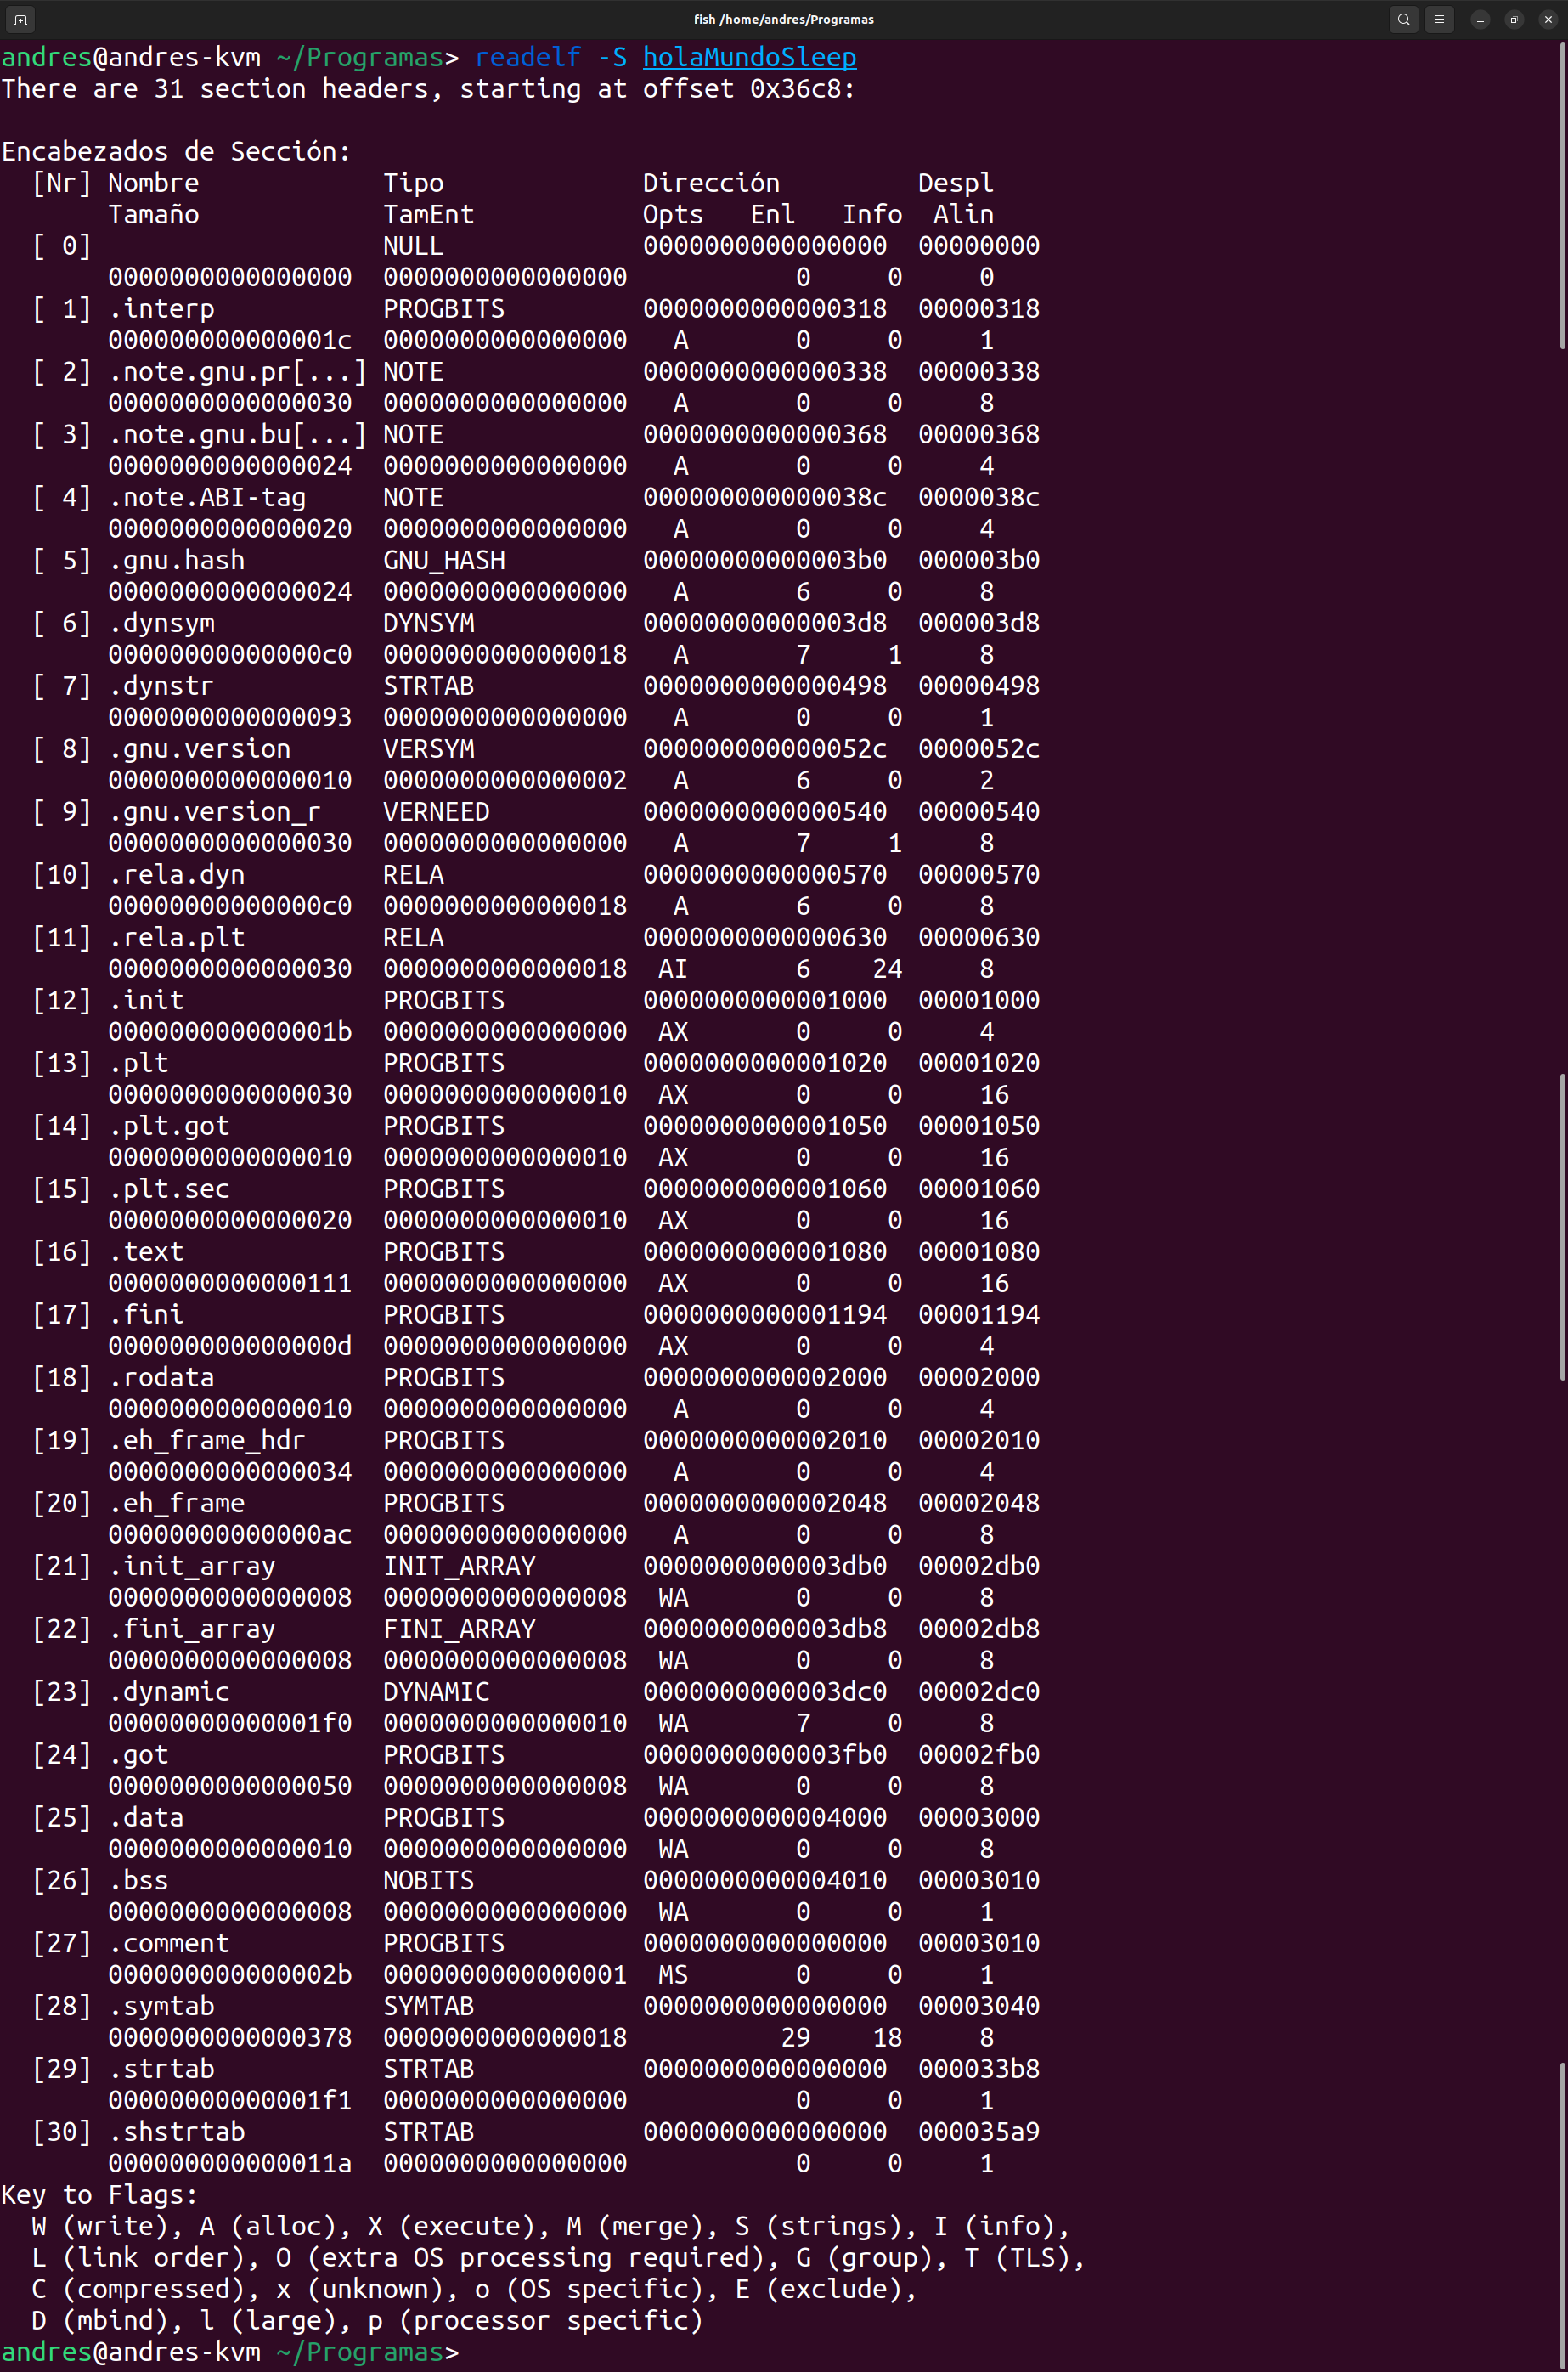
\includegraphics[width=\textwidth]{imagenes/readelfSsleep.png}
\end{figure}

\newpage

Usando la orden \verb|readelf -Wl <archivo>| se pueden obtener las cabeceras del programa.

%foto
\begin{figure}[H]
    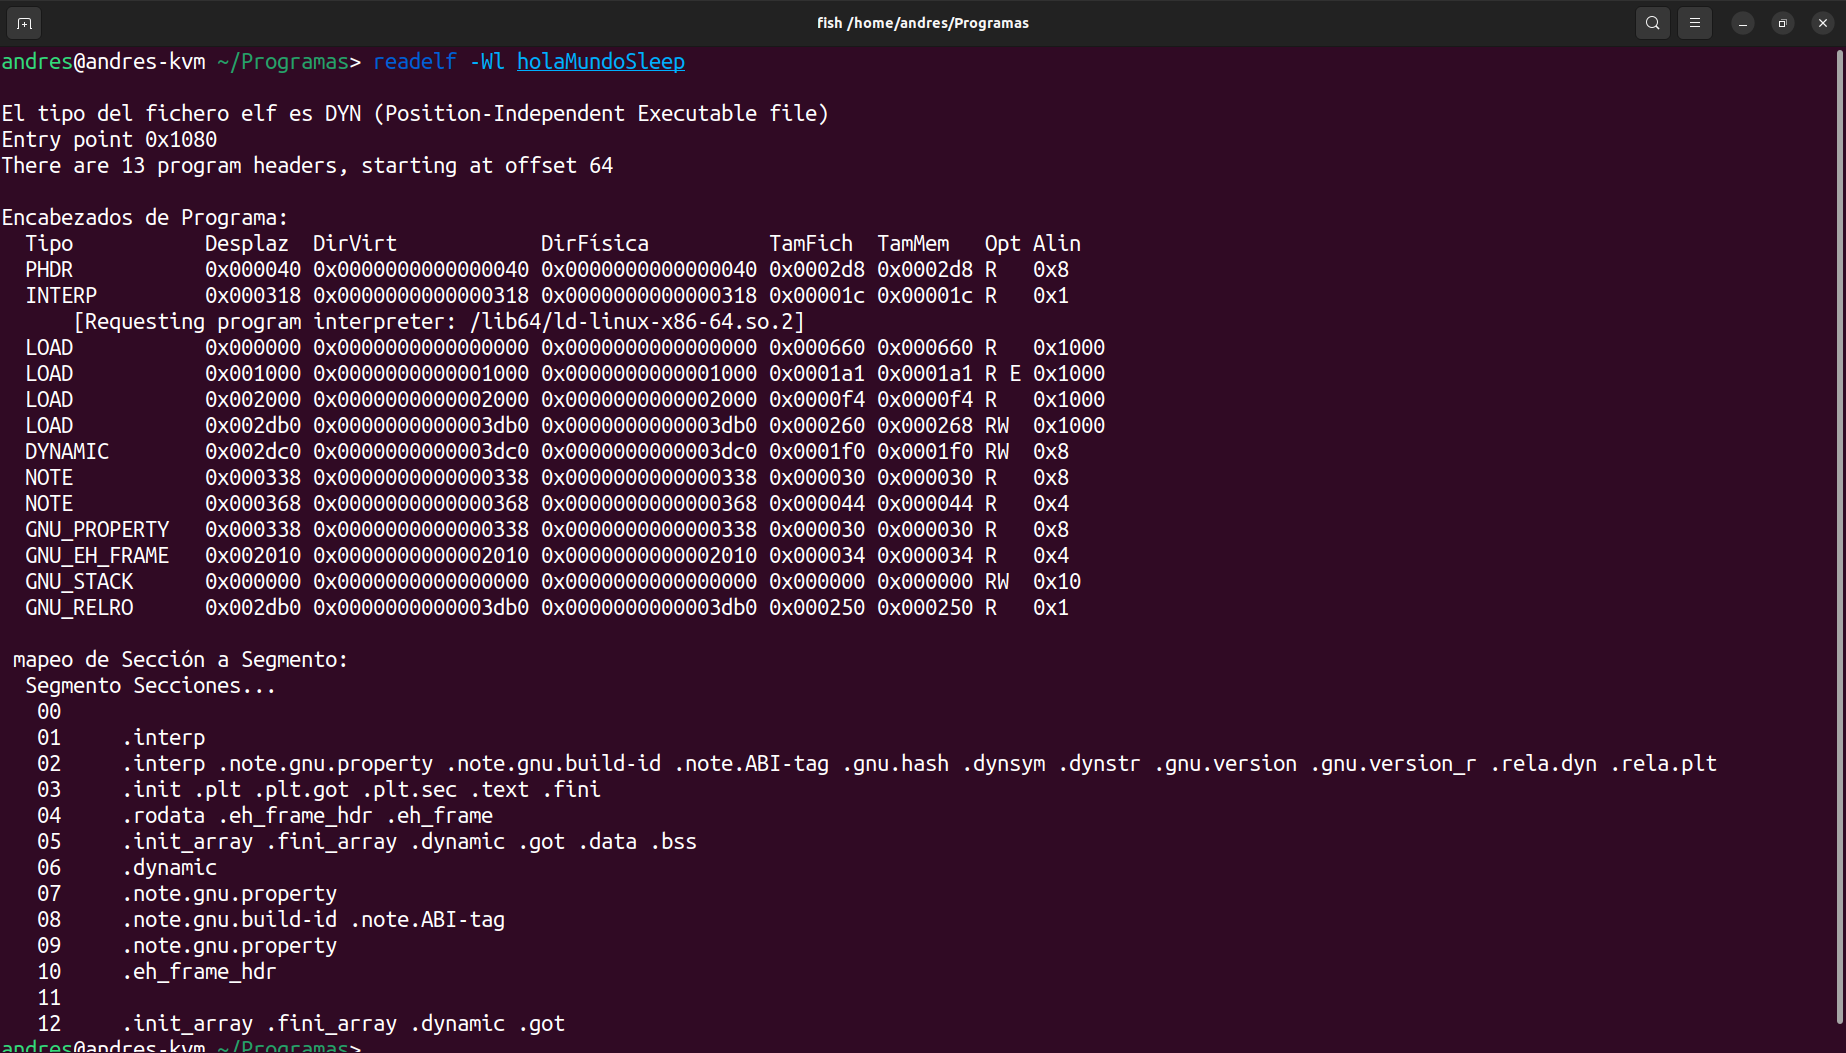
\includegraphics[width=\textwidth]{imagenes/Captura desde 2022-11-17 18-38-45.png}
\end{figure}

Como en el ejercicio anterior, la salida es la misma usando el comando \verb|objdump -p|:

%salida de objdump
\begin{figure}[H]
    \centering
    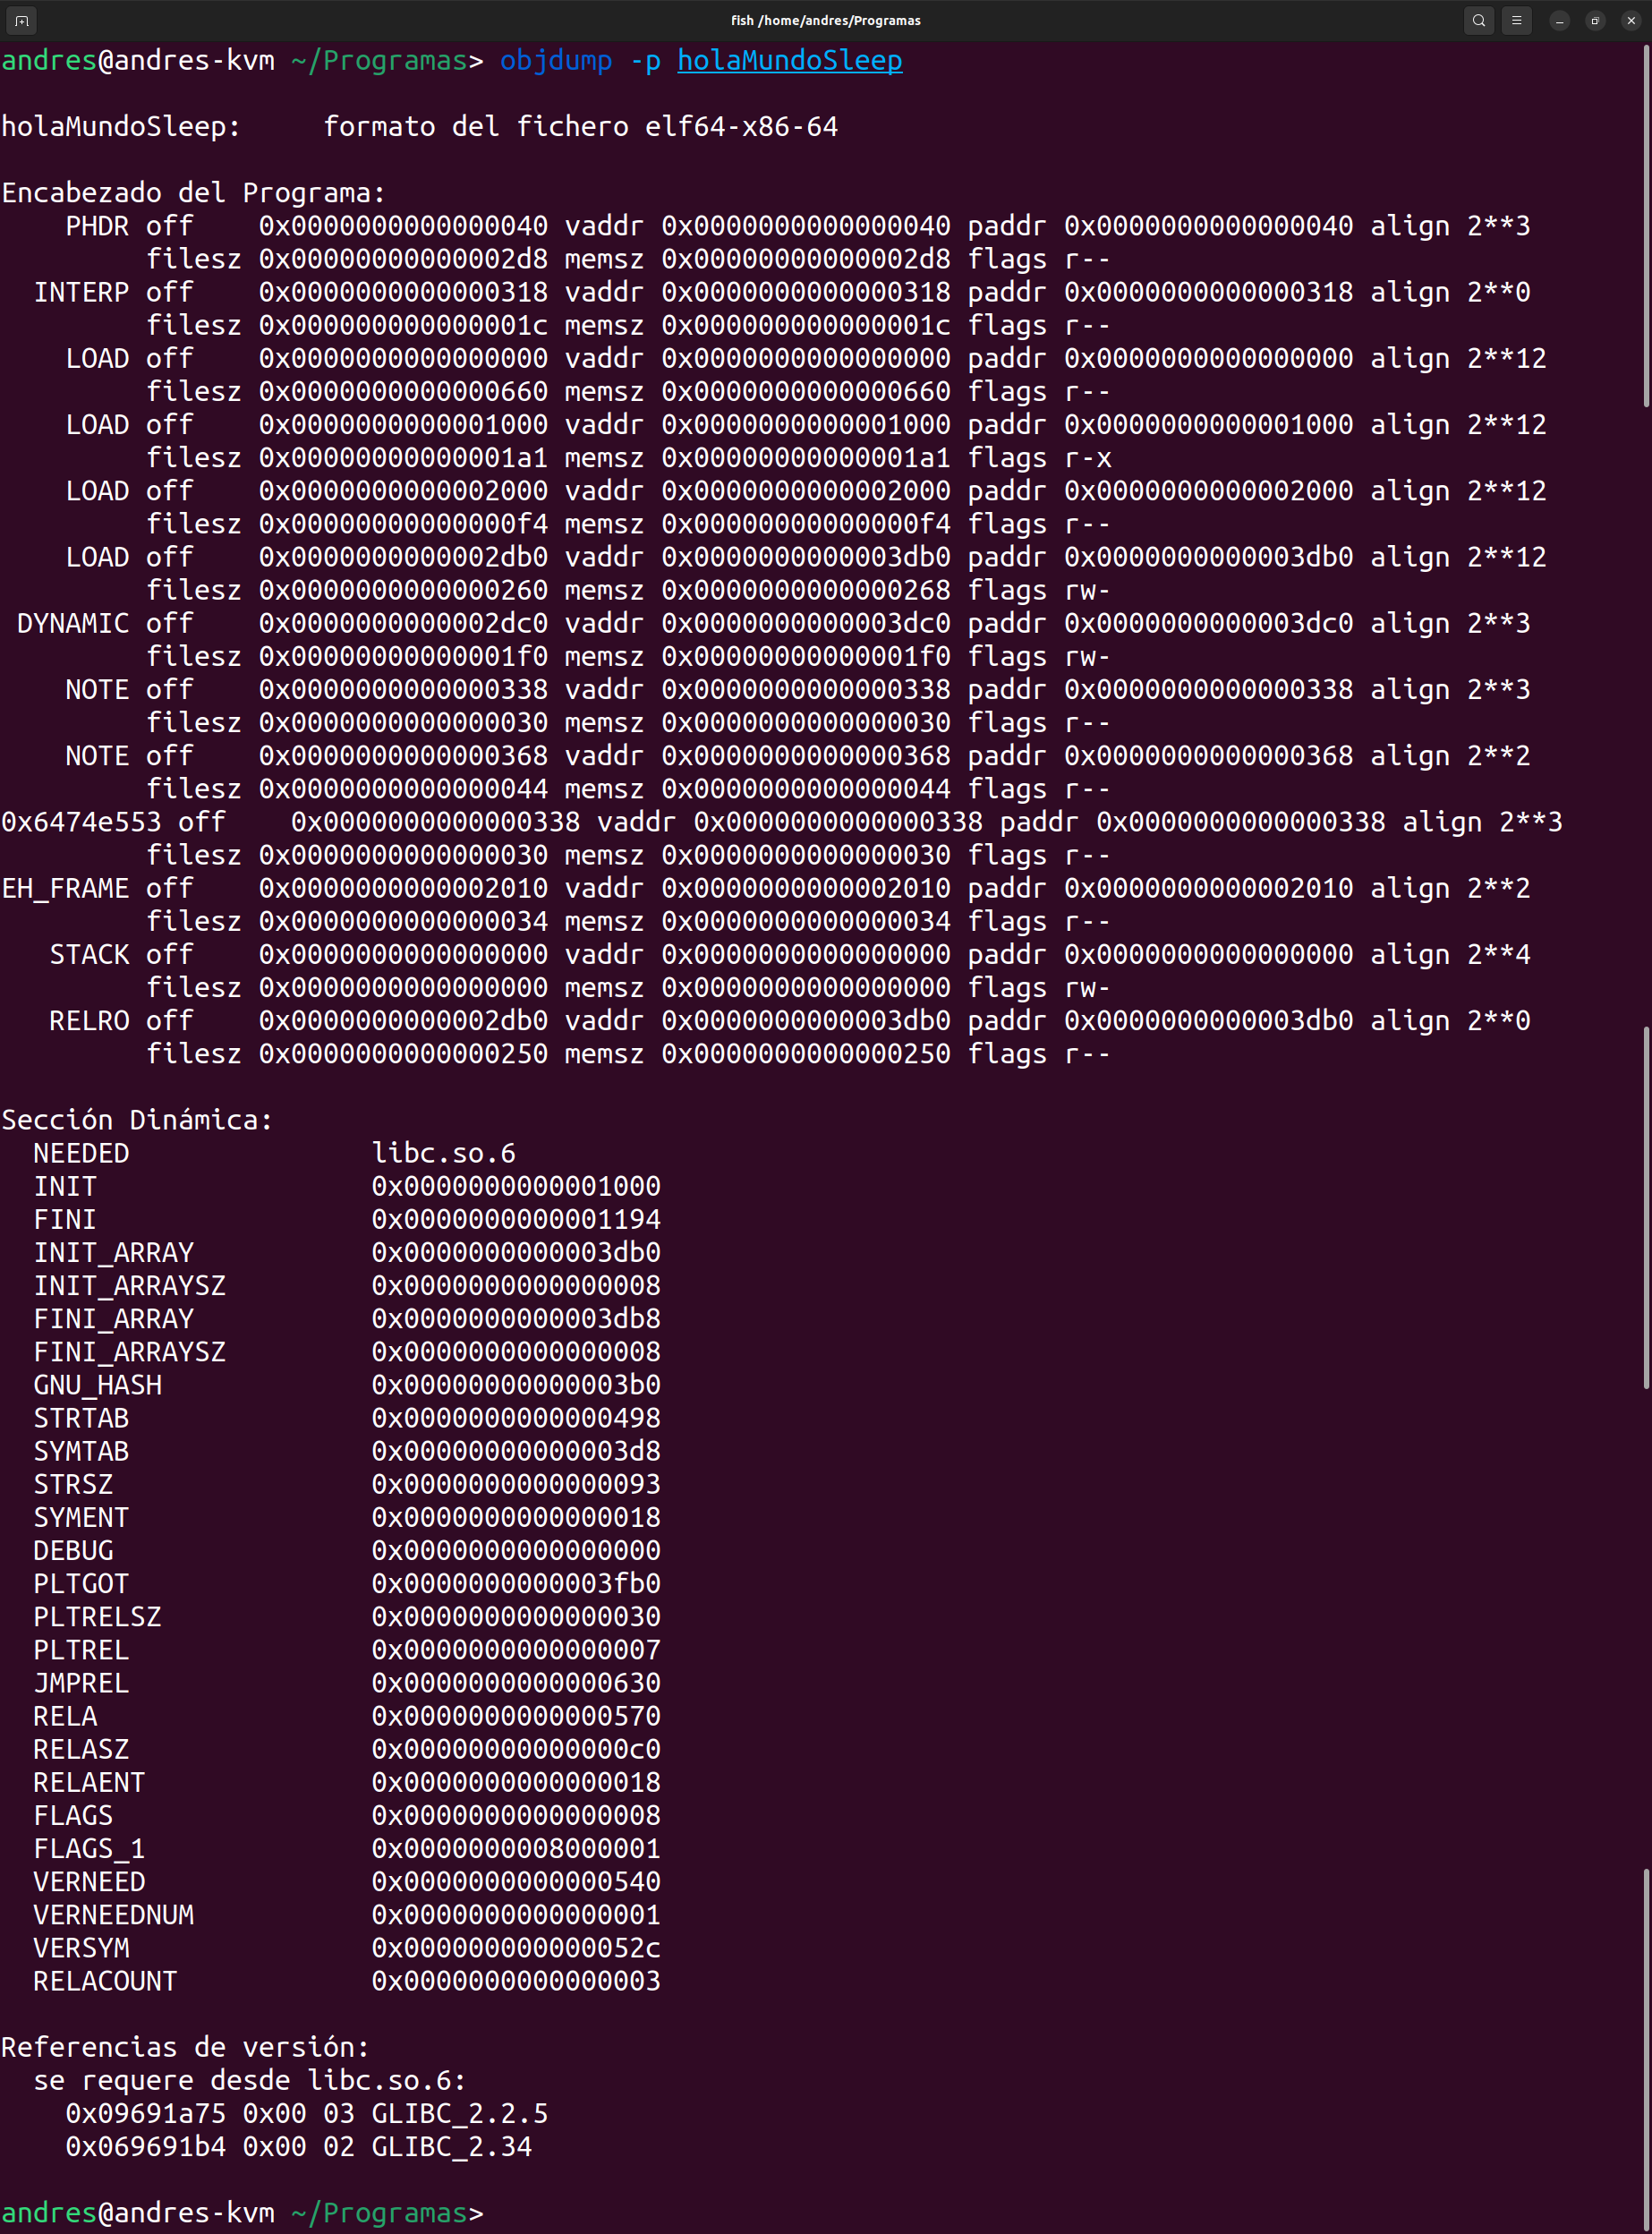
\includegraphics[width=0.7\textwidth]{imagenes/objdumppsleep.png}
\end{figure}

El kernel cuando ve \texttt{INTERP}, carga el primer \texttt{LOAD}, después los segmentos del programa interprete y finalmente se cargan las bibliotecas especificadas en \texttt{LD\_PRELOAD} y los segmentos \texttt{DYNAMIC}. 

\bigskip

Estos segmentos dinámicos que se cargan se pueden ver con la orden \verb|readelf -d <archivo>|.

%foto de la salida
\begin{figure}[H]
    \centering
    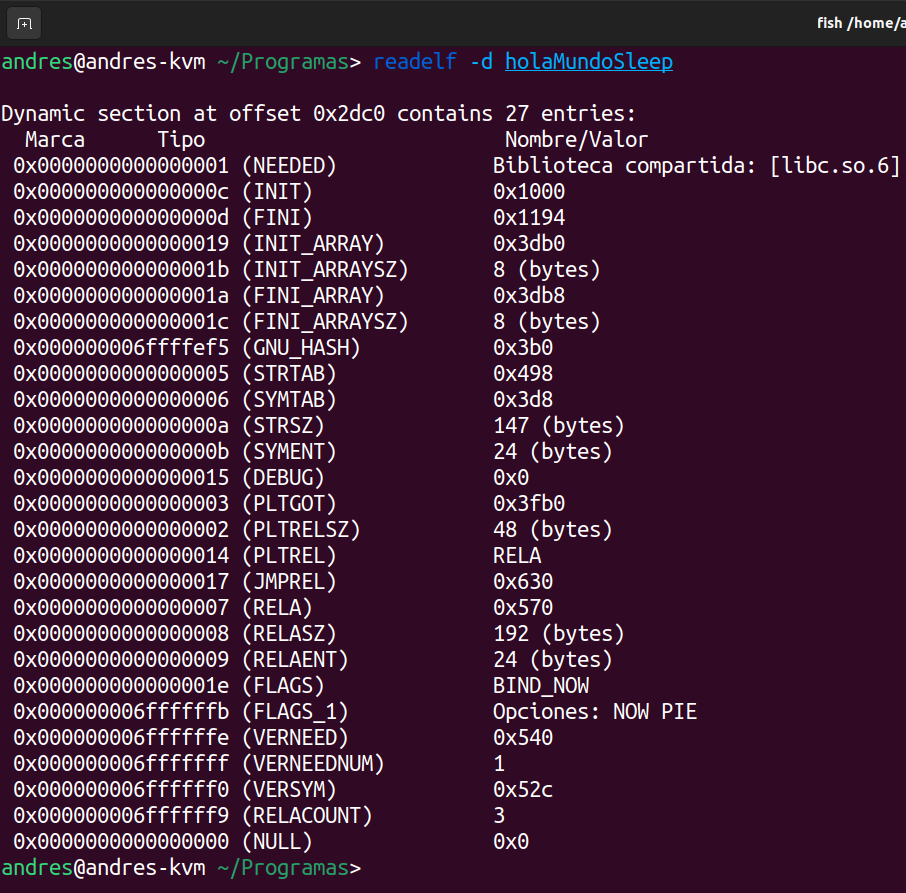
\includegraphics[width=0.7\textwidth]{imagenes/Captura desde 2022-11-17 18-47-41.png}
\end{figure}


\end{document}
